\documentclass[11pt,a4paper]{article}
\usepackage[margin=25mm]{geometry}
\usepackage[T1]{fontenc}
\usepackage[utf8]{inputenc}
\usepackage{amsmath,amssymb,graphicx,booktabs,array,longtable}
\usepackage[unicode,breaklinks=true,hidelinks]{hyperref}
\setlength{\parindent}{0pt}
\setlength{\parskip}{5pt}
\setlength{\emergencystretch}{3em}
\setlength{\tabcolsep}{3pt}
\begin{document}
\begin{center}\Large\bfseries Online Supplement: Forecasting Peak Net Positions: Known Floors, Endpoint-to-Peak Bounds and Score--Coverage Disagreement\end{center}
Detailed constructions, full outputs and diagnostics; \(\dagger\) denotes later analyses

\section*{S1. Complete report menus and robustness outputs}
\subsection*{Introduction}
We ask whether mature conditional estimators improve forecasts of an absolute sampled-position peak relative to simple historical constructions. Every report is evaluated against the same peak response and upper-quantile score on common forecast origins. The endpoint-derived bound introduced below is a benchmark rather than a direct peak-quantile estimate. The historical alternatives use past headrooms, paths translated to the current signed position, or historical peaks floored at the observed current magnitude. The conditional alternatives use ridge quantile regression, nearest-neighbor quantiles and scaled nearest-neighbor quantiles.

\subsection*{Target and forecasting methods}
\begingroup\footnotesize
\begin{samepage}Table S1. Notation. Distinct symbols for response, refits, history, distances and preferences.\end{samepage}
\begin{longtable}{>{\raggedright\arraybackslash}p{0.230\linewidth}>{\raggedright\arraybackslash}p{0.730\linewidth}}
\toprule
Symbol & Definition \\
\midrule
\endhead
\(N_t;\ B_t\) & Signed position; observed issue magnitude \(|N_t|\) \\
\(P_{t,H};\ G_{t,H}\) & Sampled absolute peak; headroom \(P_{t,H}-B_t\) \\
\(\kappa(t);\ W;\ d\) & Most recent refit index; label-pool size; refit step \\
\(C_t^m;\ \mathrm{Floor}\) & Issued report for method m; the known-floor report \\
\(d_{\rm abs};\ d_{\rm signed}\) & Common-set anchor-distance radii \\
\(\widetilde N_{i,h}^{\rm tr};\ M_{i,h}\) & Translated historical path; AR residual-replay path \\
\(a_\kappa;\ z_{i,\kappa}\) & Training response scale; standardized predictors \\
\(a;\ \omega=a/(1-a)\) & Shortfall weight; shortfall/excess preference ratio \\
\(\mathcal J_\lambda;\ \mathcal D_\lambda\) & Penalized regression objective; feasible dual objective \\
\bottomrule
\end{longtable}
\endgroup
\subsection*{Evaluation design}
\begingroup\footnotesize
\begin{samepage}Table S2. Complete validation-selected parameters. QR entries are ridge penalties; KNN entries are neighborhood counts. W52 plain KNN selects the full pool at both horizons.\end{samepage}
\begin{longtable}{>{\raggedright\arraybackslash}p{0.160\linewidth}>{\raggedright\arraybackslash}p{0.160\linewidth}>{\raggedright\arraybackslash}p{0.160\linewidth}>{\raggedright\arraybackslash}p{0.160\linewidth}>{\raggedright\arraybackslash}p{0.160\linewidth}>{\raggedright\arraybackslash}p{0.160\linewidth}}
\toprule
Source & H & W & QR \(\lambda\) & KNN k & Scaled KNN k \\
\midrule
\endhead
FX & 6 & 720 & 0.01 & 180 & 360 \\
FX & 6 & 2880 & 0.01 & 180 & 180 \\
FX & 24 & 720 & 0.01 & 180 & 180 \\
FX & 24 & 2880 & 0.001 & 180 & 180 \\
Treasury & 6 & 52 & 0.1 & 52 & 52 \\
Treasury & 6 & 260 & 0.001 & 80 & 80 \\
Treasury & 24 & 52 & 0.001 & 52 & 40 \\
Treasury & 24 & 260 & 0.1 & 160 & 160 \\
\bottomrule
\end{longtable}
\endgroup
The original conditional-study design and selected parameters were publicly frozen before their respective executions (see the linked reproduction record). The FX evaluation interval had previously been inspected. All new inference and robustness analyses are labeled post-result / exploratory; the round2 additions have local execution bindings, rather than a new public preregistration.

\subsection*{Results: FX}
\begingroup\footnotesize
\begin{samepage}Table S3. Complete selected conditional menu with breach rates and same-history frozen-F contrasts. Loss is in source-specific USD millions; B1 statistics are post-result / exploratory.\end{samepage}
\begin{longtable}{>{\raggedright\arraybackslash}p{0.137\linewidth}>{\raggedright\arraybackslash}p{0.137\linewidth}>{\raggedright\arraybackslash}p{0.137\linewidth}>{\raggedright\arraybackslash}p{0.137\linewidth}>{\raggedright\arraybackslash}p{0.137\linewidth}>{\raggedright\arraybackslash}p{0.137\linewidth}>{\raggedright\arraybackslash}p{0.137\linewidth}}
\toprule
H & W & Method & Loss & Breach rate & \(\Delta\) frozen F & DM / HLN \\
\midrule
\endhead
6 & 720 & QR & 0.433 & 8.015\% & -2.117\% & \(t=-0.616\); \(p=0.538\); HLN \(p=0.538\) \\
6 & 720 & KNN & 0.436 & 4.815\% & -1.394\% & \(t=-0.719\); \(p=0.472\); HLN \(p=0.473\) \\
6 & 720 & Scaled KNN & 0.466 & 4.060\% & +5.349\% & \(t=1.245\); \(p=0.213\); HLN \(p=0.214\) \\
6 & 2880 & QR & 0.386 & 5.675\% & -14.767\% & \(t=-5.866\); \(p=4.47\times10^{-9}\); HLN \(p=4.83\times10^{-9}\) \\
6 & 2880 & KNN & 0.411 & 4.815\% & -9.302\% & \(t=-3.615\); \(p=0.0003\); HLN \(p=0.000306\) \\
6 & 2880 & Scaled KNN & 0.426 & 4.121\% & -5.795\% & \(t=-1.255\); \(p=0.209\); HLN \(p=0.21\) \\
24 & 720 & QR & 1.035 & 13.947\% & +31.504\% & \(t=3.223\); \(p=0.00127\); HLN \(p=0.00133\) \\
24 & 720 & KNN & 0.836 & 7.592\% & +6.197\% & \(t=1.527\); \(p=0.127\); HLN \(p=0.128\) \\
24 & 720 & Scaled KNN & 0.897 & 6.642\% & +13.886\% & \(t=1.541\); \(p=0.123\); HLN \(p=0.125\) \\
24 & 2880 & QR & 0.735 & 8.015\% & -3.758\% & \(t=-0.504\); \(p=0.614\); HLN \(p=0.615\) \\
24 & 2880 & KNN & 0.770 & 6.883\% & +0.837\% & \(t=0.185\); \(p=0.854\); HLN \(p=0.854\) \\
24 & 2880 & Scaled KNN & 0.848 & 5.962\% & +11.085\% & \(t=1.325\); \(p=0.185\); HLN \(p=0.187\) \\
\bottomrule
\end{longtable}
\endgroup
\subsection*{Results: Treasury}
\begingroup\footnotesize
\begin{samepage}Table S4. Complete selected conditional menu with breach rates and same-history frozen-F contrasts. Loss is in source-specific USD millions; B1 statistics are post-result / exploratory.\end{samepage}
\begin{longtable}{>{\raggedright\arraybackslash}p{0.137\linewidth}>{\raggedright\arraybackslash}p{0.137\linewidth}>{\raggedright\arraybackslash}p{0.137\linewidth}>{\raggedright\arraybackslash}p{0.137\linewidth}>{\raggedright\arraybackslash}p{0.137\linewidth}>{\raggedright\arraybackslash}p{0.137\linewidth}>{\raggedright\arraybackslash}p{0.137\linewidth}}
\toprule
H & W & Method & Loss & Breach rate & \(\Delta\) frozen F & DM / HLN \\
\midrule
\endhead
6 & 52 & QR & 5095.519 & 30.325\% & +83.354\% & \(t=3.057\); \(p=0.00224\); HLN \(p=0.00298\) \\
6 & 52 & KNN & 2779.054 & 3.971\% & +0.000\% & IDENTICAL\_LOSSES \\
6 & 52 & Scaled KNN & 4208.293 & 3.249\% & +51.429\% & \(t=3.682\); \(p=0.000231\); HLN \(p=0.000365\) \\
6 & 260 & QR & 4159.673 & 19.495\% & +50.786\% & \(t=2.669\); \(p=0.00761\); HLN \(p=0.00939\) \\
6 & 260 & KNN & 2663.561 & 10.108\% & -3.447\% & \(t=-0.442\); \(p=0.658\); HLN \(p=0.665\) \\
6 & 260 & Scaled KNN & 3127.173 & 8.303\% & +13.358\% & \(t=0.945\); \(p=0.345\); HLN \(p=0.355\) \\
24 & 52 & QR & 12165.574 & 47.653\% & +227.411\% & \(t=2.238\); \(p=0.0252\); HLN \(p=0.0415\) \\
24 & 52 & KNN & 3715.693 & 11.913\% & +0.000\% & IDENTICAL\_LOSSES \\
24 & 52 & Scaled KNN & 5625.667 & 11.552\% & +51.403\% & \(t=2.797\); \(p=0.00516\); HLN \(p=0.011\) \\
24 & 260 & QR & 5204.760 & 30.325\% & +109.843\% & \(t=1.667\); \(p=0.0955\); HLN \(p=0.128\) \\
24 & 260 & KNN & 2257.963 & 4.693\% & -8.964\% & \(t=-1.941\); \(p=0.0523\); HLN \(p=0.0768\) \\
24 & 260 & Scaled KNN & 4137.264 & 2.888\% & +66.805\% & \(t=4.923\); \(p=8.53\times10^{-7}\); HLN \(p=9.8\times10^{-6}\) \\
\bottomrule
\end{longtable}
\endgroup
\subsection*{Robustness}
AR has lower loss in five of eight cells against S, five against F and five against QR; these sets differ. Relative to QR it loses in three of four FX cells and improves in all four Treasury cells. The exploratory AR comparisons show a different observed loss pattern from the adverse Treasury QR primary. Against S, the FX H6 changes are \(-\)1.536\%/\(-\)0.546\% at W720/W2880, while H24 changes are +2.386\%/+5.147\%. Treasury changes are \(-\)13.444\%/\(-\)18.887\% at H6 and +35.125\%/\(-\)24.118\% at H24 for W52/W260. The complete table retains the original model identities. Against S, AR mean report and mean overprediction amount decrease in every cell, while strict breach occasions increase in all eight and mean underprediction amount increases in seven. Treasury H24 W260 loss falls from 2478.871 to 1881.016 USD millions (\(-\)24.118\%), yet breaches rise from 12 to 59 of 277 and mean underprediction amount rises from 306.848 to 892.437. Mean unused allowance falls from 43747.307 to 20664.031. Under the stipulated score, .05 times the unused reduction exceeds .95 times the added overrun. This explains the observed loss change without asserting safer limits, calibrated tails or observed financing savings.

A later post-inspection rank/endpoint ablation adds a same-pool, same-update intercept-only empirical headroom quantile, choosing its lower minimizer endpoint. The matched FX H6 W2880 QR comparison still lowers loss by 14.773\%, with 376 rather than 365 breaches; the matched Treasury H6 W260 QR comparison still raises loss by 46.058\%, with 54 rather than 32 breaches. All four Treasury QR cells remain adverse against this added report. The lower-rank rule improves on original frozen F in three cells and loses in five, so the empirical minimizer endpoint can perform worse in evaluation. The two headline signs persist under this specific control. Table S17 retains every cell and the later design history.

Post-result diagnostics clarify the issued reports rather than changing their rankings. Every common realized target satisfies \(P(H6)\le P(H24)\), yet the separately fitted reports can cross: FX W720 QR crosses on 640/6,625 issues, and Treasury W52 QR on 91/277. Some short Treasury historical F/S controls also cross because the horizons use different mature episode sets. Supplement S5 retains all 45 original pairs and a separately frozen addition covering all four AR pairs. AR has zero observed FX crossings, but Treasury W52/W260 cross on 59/26 of 277 issues. The horizon-specific fits and mature scenario sets differ, producing the observed incoherence. Supplement Figure S3 retains the complete annual comparison; all detailed coherence and fixed-terminal diagnostics remain in Supplement S5.

\begingroup\footnotesize
\begin{samepage}Table S5\(\dagger\). Summary of post-result / exploratory robustness; complete numerical tables remain in the appendices.\end{samepage}
\begin{longtable}{>{\raggedright\arraybackslash}p{0.180\linewidth}>{\raggedright\arraybackslash}p{0.410\linewidth}>{\raggedright\arraybackslash}p{0.370\linewidth}}
\toprule
Analysis & Main finding & Retained adverse evidence \\
\midrule
\endhead
AR replay & Improves on QR in every Treasury cell & Breach occasions rise against S in every cell \\
Empirical rank & Both matched H6 QR directions persist & Lower empirical rank loses to F in five cells \\
Preference frontier & FX H6 reduces both loss components & FX H24 reverses near the original weight \\
Horizon coherence & Targets are ordered by construction & Separately fitted reports cross \\
\bottomrule
\end{longtable}
\endgroup
\begingroup\footnotesize
\begin{samepage}Table S6\(\dagger\). Post-result / exploratory paired predictive-accuracy tests. Negative t favors QR; normal DM and Student-reference HLN p values are two sided. Holm p uses the fixed 72 common-history family; original cross-window FX comparisons are outside it. Original primaries and legacy remain fixed.\end{samepage}
\begin{longtable}{>{\raggedright\arraybackslash}p{0.200\linewidth}>{\raggedright\arraybackslash}p{0.080\linewidth}>{\raggedright\arraybackslash}p{0.090\linewidth}>{\raggedright\arraybackslash}p{0.090\linewidth}>{\raggedright\arraybackslash}p{0.120\linewidth}>{\raggedright\arraybackslash}p{0.190\linewidth}>{\raggedright\arraybackslash}p{0.170\linewidth}}
\toprule
Comparison & L & DM t & DM p & HLN t & HLN p & Holm p \\
\midrule
\endhead
FX H6 primary & 10 & -5.18 & 2.2e-07 & -5.18 & 2.31e-07 & Outside family \\
FX H6 matched & 10 & -5.87 & 4.47e-09 & -5.86 & 4.83e-09 & 2.86e-07 \\
FX H24 legacy & 24 & -0.204 & 0.839 & -0.203 & 0.839 & Outside family \\
Treasury H6 primary & 6 & 2.67 & 0.00761 & 2.62 & 0.00939 & 0.32 \\
\bottomrule
\end{longtable}
\endgroup
\begingroup\footnotesize
\begin{samepage}Table S7\(\dagger\). Post-result / exploratory parsimonious QR. Four predictors plus intercept, expanded validation penalty menu, original split/refit schedule. Percent changes compare loss against the original QR and matched F. Every original primary remains unchanged.\end{samepage}
\begin{longtable}{>{\raggedright\arraybackslash}p{0.120\linewidth}>{\raggedright\arraybackslash}p{0.120\linewidth}>{\raggedright\arraybackslash}p{0.120\linewidth}>{\raggedright\arraybackslash}p{0.120\linewidth}>{\raggedright\arraybackslash}p{0.120\linewidth}>{\raggedright\arraybackslash}p{0.120\linewidth}>{\raggedright\arraybackslash}p{0.120\linewidth}>{\raggedright\arraybackslash}p{0.120\linewidth}}
\toprule
Source & H & W & \(\lambda\) & \(\Delta\) QR \% & \(\Delta\) F \% & Breaches & Status \\
\midrule
\endhead
Treasury & 6 & 52 & 10 & -46.9 & -2.59 & 15 & COMPLETE \\
Treasury & 6 & 260 & 10 & -32.2 & 2.17 & 32 & COMPLETE \\
Treasury & 24 & 52 & 10 & -67.6 & 5.95 & 36 & COMPLETE \\
Treasury & 24 & 260 & 10 & -52.3 & 0.11 & 15 & COMPLETE \\
FX & 6 & 720 & 0.01 & 3.67 & 1.48 & 414 & COMPLETE \\
FX & 6 & 2880 & 0.01 & 12.3 & -4.29 & 399 & COMPLETE \\
FX & 24 & 720 & 0.01 & -11.4 & 16.5 & 701 & COMPLETE \\
FX & 24 & 2880 & 0.01 & 0.898 & -2.89 & 508 & COMPLETE \\
\bottomrule
\end{longtable}
\endgroup
\begingroup\footnotesize
\begin{samepage}Table S8\(\dagger\). All eight classical-bound plug-in L cells. Loss uses source-native units (FX USD; Treasury USD millions). \(\Delta\) F/QR compares the same W and refit schedule; positive values are adverse for L. DM p is the unadjusted working-reference paired L--F test; Supplement S11 retains both comparators and a separate 16-member Holm family. Original primaries are unchanged.\end{samepage}
\begin{longtable}{>{\raggedright\arraybackslash}p{0.120\linewidth}>{\raggedright\arraybackslash}p{0.120\linewidth}>{\raggedright\arraybackslash}p{0.120\linewidth}>{\raggedright\arraybackslash}p{0.120\linewidth}>{\raggedright\arraybackslash}p{0.120\linewidth}>{\raggedright\arraybackslash}p{0.120\linewidth}>{\raggedright\arraybackslash}p{0.120\linewidth}>{\raggedright\arraybackslash}p{0.120\linewidth}}
\toprule
Source & H & W & Mean loss & Hits / n & \(\Delta\) F \% & \(\Delta\) QR \% & DM p vs F \\
\midrule
\endhead
FX & 6 & 720 & 5.795e+05 & 101/6625 & 30.93 & 33.76 & 2.988e-15 \\
FX & 6 & 2880 & 5.903e+05 & 75/6625 & 30.39 & 52.98 & 6.695e-15 \\
FX & 24 & 720 & 8.728e+05 & 136/6625 & 10.85 & -15.71 & 0.06462 \\
FX & 24 & 2880 & 8.24e+05 & 174/6625 & 7.941 & 12.16 & 0.03958 \\
Treasury & 6 & 52 & 2873 & 10/277 & 3.37 & -43.62 & 0.3317 \\
Treasury & 6 & 260 & 2434 & 15/277 & -11.77 & -41.49 & 0.1785 \\
Treasury & 24 & 52 & 4694 & 42/277 & 26.32 & -61.42 & 0.1167 \\
Treasury & 24 & 260 & 2725 & 22/277 & 9.868 & -47.64 & 0.2746 \\
\bottomrule
\end{longtable}
\endgroup
\begingroup\footnotesize
\begin{samepage}Table S9\(\dagger\). Complete panel summary: number of four H/W cells with lower pinball loss than matched F. These are descriptive counts, not independent trials or evidence selected after screening losses. Supplement S12 retains every loss change and breach count.\end{samepage}
\begin{longtable}{>{\raggedright\arraybackslash}p{0.240\linewidth}>{\raggedright\arraybackslash}p{0.240\linewidth}>{\raggedright\arraybackslash}p{0.240\linewidth}>{\raggedright\arraybackslash}p{0.240\linewidth}}
\toprule
Series key & QR33 lower / cells & C2 lower / cells & L lower / cells \\
\midrule
\endhead
PDPOSMBS-TOT & 0/4 & 0/4 & 2/4 \\
PDPOSCS-TOT & 0/4 & 3/4 & 1/4 \\
PDPOSFGS-TOT & 1/4 & 1/4 & 3/4 \\
PDPOSTIPS-L2 & 0/4 & 0/4 & 4/4 \\
PDPOSTIPS-G11 & 0/4 & 0/4 & 1/4 \\
PDPOSTIPS-G2 & 0/4 & 0/4 & 0/4 \\
PDPOSTIPS-G6L11 & 2/4 & 4/4 & 0/4 \\
PDPOSGSC-L2 & 0/4 & 2/4 & 2/4 \\
PDPOSGSC-G2L3 & 0/4 & 0/4 & 2/4 \\
PDPOSGSC-G3L6 & 0/4 & 0/4 & 2/4 \\
PDPOSGSC-G6L7 & 0/4 & 0/4 & 1/4 \\
PDPOSGSC-G7L11 & 0/4 & 1/4 & 1/4 \\
\bottomrule
\end{longtable}
\endgroup
\begingroup\footnotesize
\begin{samepage}Table S10\(\dagger\). Fixed FHS, GARCH-scaled peak-headroom POT and true leaf-distribution QRF on all original cells. Each entry gives \(\Delta\) loss\% versus matched frozen F / strict breaches; negative \(\Delta\) favors the new method. NA retains a failed or structurally ineligible complete-cell comparison; issued counts are not scored as partial successes. Full native losses, reasons and comparisons are in Supplement S13.\end{samepage}
\begin{longtable}{>{\raggedright\arraybackslash}p{0.160\linewidth}>{\raggedright\arraybackslash}p{0.160\linewidth}>{\raggedright\arraybackslash}p{0.160\linewidth}>{\raggedright\arraybackslash}p{0.160\linewidth}>{\raggedright\arraybackslash}p{0.160\linewidth}>{\raggedright\arraybackslash}p{0.160\linewidth}}
\toprule
Source & H & W & FHS: \(\Delta\)\% / hits & Peak POT: \(\Delta\)\% / hits & QRF: \(\Delta\)\% / hits \\
\midrule
\endhead
FX & 6 & 720 & NA (240 issued) & NA (240 issued) & 5.793 / 402 \\
FX & 6 & 2880 & -1.258 / 278 & 3.269 / 363 & -4.48 / 354 \\
FX & 24 & 720 & NA (240 issued) & NA (240 issued) & 16.02 / 779 \\
FX & 24 & 2880 & 6.255 / 136 & 10.61 / 369 & 7.335 / 600 \\
Treasury & 6 & 52 & -1.883 / 7 & NA (0 issued) & -6.83 / 16 \\
Treasury & 6 & 260 & -8.276 / 4 & -10.35 / 17 & 6.198 / 33 \\
Treasury & 24 & 52 & 60.26 / 0 & NA (0 issued) & 4.279 / 44 \\
Treasury & 24 & 260 & 125.1 / 0 & 32.09 / 20 & 33.94 / 62 \\
\bottomrule
\end{longtable}
\endgroup
\subsection*{Discussion and limitations}
The FX evaluation interval was previously inspected, and the subsequent robustness analyses are post-result / exploratory. These records do not restore a compatible unseen dealer sample. Treasury is a downloaded-vintage, economic-date aggregate replay rather than an original-release public-information backtest; cross-dealer netting, valuation and composition distinguish it from an individual dealer's book.

The annual decomposition is a readback of published aggregates. Year-specific paired mean differences are weighted by their origin counts before computing contribution shares; annual percentage improvements are not averaged. Exact rational arithmetic operates on saved decimal tokens and does not recover infinite-precision original individual losses. The archived annual-decomposition receipt and helper retain source hashes, reconciliation tolerances and observed differences.

\section*{S2. Finite geometry and its predictive limits}
On a common set and fixed rank, let \(d_{\rm abs}=\max_{i\in J}\bigl|B-|N_i|\bigr|\) and \(d_{\rm signed}=\max_{i\in J}|x-N_i|\). Elementary order-statistic and projection stability gives \(|F-K|\le d_{\rm abs}\), \(|S-K|\le d_{\rm signed}\), hence \(|F-S|\le d_{\rm abs}+d_{\rm signed}\). Supplement S2 proves these finite relationships and their predictive limits. Nearest signed-state membership minimizes its maximum signed distance at a given count; it need not minimize forecast loss. These statements do not automatically bound QR, scaled responses or the richer 33-coordinate distance.

\subsection*{S2.1. common-set projection bounds}
These construction arguments concern F/S/K on an identical historical set and rank. They are retained from the earlier comparison. A one-dimensional signed-distance minimax property does not extend automatically to the multivariate neighbor distance, and the bounds do not automatically constrain QR or scale-adjusted responses.

These are elementary finite-array arguments, rather than new asymptotic or coverage results. Fix a nonempty common selected set J, an available rank \(1\le k\le|J|\), query \(x=N_t\), floor \(B=|x|\) and completed historical windows. All identities in this appendix concern real arithmetic. Write \(B_i=|N_i|\), \(d_{i,h}=N_{i+h}-N_i\), with \(d_{i,0}=0\), and define

Let \(a_i=\min_h d_{i,h}\) and \(b_i=\max_h d_{i,h}\), so \(a_i\le0\le b_i\). These are the lower and upper increments denoted l and u in Section 4. The auxiliary nonnegative envelope coordinates below use \(u_i=b_i\) and \(v_i=-a_i\).

\[
A_i=B+P_i-B_i,\qquad T_i=\max_{0\le h\le H}|x+d_{i,h}|,\qquad C_B(z)=\max(B,z).
\]
Both \(A_i\) and \(T_i\) are at least B. The projection \(C_B\) is nondecreasing and 1-Lipschitz. It commutes with a finite order statistic, as does a common translation. Hence \(F_J=Q_k(A)\), \(S_J=Q_k(T)\) and \(K_J=Q_k(C_B(P))\). Since \(C_B(A_i)=A_i\),

\[
|A_i-C_B(P_i)|\le |A_i-P_i|=|B-B_i|.
\]
The reverse triangle inequality bounds each path value's change under a starting-position translation by \(|x-N_i|\). Taking a maximum gives \(|T_i-P_i|\le|x-N_i|\). Applying the same floor projection preserves that bound because \(T_i\ge B\). Finally, paired order statistics are nonexpansive in the maximum coordinate difference: if \(|u_i-v_i|\le r\) for every i, then \(u_i\le v_i+r\) and conversely; monotonicity and common translation give \(|Q_k(u)-Q_k(v)|\le r\). These observations prove the two common-set K bounds stated above. The triangle inequality and \(\bigl||N_i|-|x|\bigr|\le|N_i-x|\) prove the stated F/S bound. Keeping the rank fixed while changing one side's historical rows does not by itself justify these common-set comparison bounds.

Among all size-m subsets, selecting the m smallest signed distances minimizes the largest selected distance: any alternative must include an element at least as far away as the mth ordered distance. This finite minimax fact, with the declared tie convention, concerns the signed radius. It does not minimize the absolute-anchor radius, the sum of the two radii, the actual report gap or a forecast loss. For every fixed realized y, pinball loss is \(\max(\tau,1-\tau)\)-Lipschitz in its report, so a report-gap bound also bounds the absolute loss difference. Such stability supplies no sign for the realized or expected loss difference.

\subsection*{S2.2. envelope plateaus and the role of signed anchors}
Put \(u_i=b_i\ge0\) and \(v_i=-a_i\ge0\). The headroom of an increment envelope at any anchor z is

\[
g_i(z)=\max(z+u_i,-z+v_i)-|z|=\begin{cases}\max(u_i,v_i-2z),&z\ge0,\\\max(u_i+2z,v_i),&z\le0.\end{cases}
\]
F pools each envelope's headroom at its historical anchor, \(g_i(N_i)\); S pools its headroom at the query, \(g_i(x)\). The branches agree at zero and together make \(g_i\) 2-Lipschitz, with range lying in \([\min(u_i,v_i),\max(u_i,v_i)]\). Apply the distance and range bounds to each paired row, then use the same-rank order-statistic stability from S2.1 to obtain

\[
|F_J-S_J|\le\max_{i\in J}\min\{2|x-N_i|,|u_i-v_i|\}.
\]
For example, \(u_i=v_i\) in every row makes \(F_J=S_J\) at arbitrary anchors. Nonnegative query/source anchors together with \(u_i\ge v_i\) in every row also suffice; the nonpositive analogue uses \(v_i\ge u_i\). These are sufficient conditions, not a characterization: pooled order statistics can coincide even when paired rows differ. The range bound also gives \(F_J,S_J\le R_J\), where \(R_J=B+Q_k\{\max(u_i,v_i):i\in J\}\). This is a theoretical same-set ordering; no R retrieval configuration is evaluated in the extension, and the ordering does not make \(R_J\) preferable under a given loss.

If every \(B_i\le B\), then \(A_i\ge C_B(P_i)\) and \(F_J\ge K_J\). If every \(B_i\ge B\), then \(C_B(P_i)=P_i\ge A_i\) and \(F_J\le K_J\). Equal absolute anchors force F=K but leave signs relevant to S. A coherent full-pool example uses \(c>0\), \(H=1\), \(n=720\), \(\tau=19/20\), \(t=721\) and \(N_s=(-1)^{s+1}c\) for \(0\le s\le721\). The pool uses completed labels at origins \(J=\{1,\ldots,720\}\), with 360 anchors of each sign and current \(N_t=c\). All historical peaks equal c and headrooms equal zero, so F=K=c. Raw reanchoring gives 360 peaks c and 360 peaks 3c; rank 685 gives S=3c. Thus \(d_{\rm abs}=0\) while \(d_{\rm signed}=2c\) and \(|S-K|=2c\). This artificial path respects maturity and an available corrected rank; it is not an empirical claim or a claim about which rows nearest retrieval selects.

\subsection*{S2.3. the same observed history allows opposite loss rankings}
Choose \(d>0\), \(H\ge 1\), \(0<\tau<1\) and n large enough that \(k=\lceil(n+1)\tau\rceil\le n\). Set \(t=H+n-1\) and \(N_s=d(t-s)\) for \(0\le s\le t\), using \(J=\{0,\ldots,n-1\}\). Every selected response ends by t. Each historical peak is its own positive starting value, so \(G_i=0\) and \(F=0\). Each increment path equals \(-dh\); reanchoring at \(N_t=0\) gives \(S=Hd\). Two continuations of this identical observed history yield:

\begingroup\footnotesize
\begin{samepage}Table S11. Artificial coherent continuations. Symbols are constructed quantities, not source-record estimates.\end{samepage}
\begin{longtable}{>{\raggedright\arraybackslash}p{0.240\linewidth}>{\raggedright\arraybackslash}p{0.240\linewidth}>{\raggedright\arraybackslash}p{0.240\linewidth}>{\raggedright\arraybackslash}p{0.240\linewidth}}
\toprule
Future \(N_{t+h}\), \(1\le h\le H\) & Actual peak & F loss & S loss \\
\midrule
\endhead
0 & 0 & 0 & \((1-\tau)Hd\) \\
\(-dh\) & \(Hd\) & \(\tau Hd\) & 0 \\
\bottomrule
\end{longtable}
\endgroup
Either report can therefore have strictly smaller realized loss under a compatible future. A report ordering also need not hold universally. Consider the artificial history (0,\(-\)4,\(-\)1,2), with \(H=1\), \(n=3\), \(\tau=3/4\), issue \(t=3\) and \(J=\{0,1,2\}\). The current anchor and floor are \(x=B=2\); all three historical windows are completed. Table S12 shows the native and raw-reanchored paths.

\begingroup\footnotesize
\begin{samepage}Table S12. Completed \(H=1\) windows from one artificial history, in arbitrary position units. P is the historical peak, G the native headroom and T the peak after reanchoring at \(x=2\). These values are not source-record estimates.\end{samepage}
\begin{longtable}{>{\raggedright\arraybackslash}p{0.160\linewidth}>{\raggedright\arraybackslash}p{0.160\linewidth}>{\raggedright\arraybackslash}p{0.160\linewidth}>{\raggedright\arraybackslash}p{0.160\linewidth}>{\raggedright\arraybackslash}p{0.160\linewidth}>{\raggedright\arraybackslash}p{0.160\linewidth}}
\toprule
i & Historical pair & P & G & Reanchored pair & T \\
\midrule
\endhead
0 & 0, \(-\)4 & 4 & 4 & 2, \(-\)2 & 2 \\
1 & \(-\)4, \(-\)1 & 4 & 0 & 2, 5 & 5 \\
2 & \(-\)1, 2 & 2 & 1 & 2, 5 & 5 \\
\bottomrule
\end{longtable}
\endgroup
The available corrected rank is \(\lceil(3+1)\cdot3/4\rceil=3\). The third order statistics of G, \(T-B\) and P are 4, 3 and 4, respectively, so \(F=6\), \(S=5\) and \(K=4\). The small pool and \(\tau=3/4\) belong only to this illustration. It contains no observation after issue and gives no realized query loss. These constructions support logical limits, not the conditional law of the recorded series or a population ranking. A deterministic construction can refute an unconditional mathematical assertion while supplying no empirical validation for either rule.

\subsection*{S2.4. raw translation versus fixed-coefficient residual replay}
For interpretation, fix arbitrary coefficients c and \(\phi\) and define residuals \(\varepsilon_s=N_{s+1}-c-\phi N_s\). Replay a historical window's ordered residuals from query x. The coefficients are fixed after a refit; this algebra does not assert a true dynamic law or a martingale-difference property. Denote replay by M and raw translation by \(\widetilde N^{\rm tr}\). Subtracting the recursions and using induction gives

\[
M_{i,h}(x)=N_{i+h}+\phi^h(x-N_i),\qquad \widetilde N^{tr}_{i,h}(x)=N_{i+h}+(x-N_i).
\]
Taking the maximum absolute path value yields

\[
\left|\max_h|\widetilde N^{tr}_{i,h}(x)|-\max_h|M_{i,h}(x)|\right|\le\max_{0\le h\le H}|1-\phi^h|\,|x-N_i|.
\]
For \(0\le\phi\le1\) the coefficient is \(1-\phi^H\); at \(\phi=1\) the paths coincide. The identity needs no residual law, while treating past residuals as representative of future conditional residuals is a separate assumption. Supplement S7 fits a specified mean recursion and compares realized loss, but does not validate that conditional residual-representativeness assumption. The extrema suffice to evaluate the peak after raw translation, but generally not after the dynamic correction, which depends on path order. The same-rank reports inherit a deterministic bound with max over historical anchor distances, not a guaranteed sign of loss improvement. Conditional validity remains a separate question.

\section*{S3. Earlier construction and retrieval evidence}
This appendix preserves the complete loss menus of the 21 October historical studies. Monetary displays are source-reported FX USD millions. The original rules include headroom F, raw reanchoring S, a symmetric increment envelope R, historical peak K (native-peak K), and the current-floor report Floor. One factor changes from the original H6/W720/\(\tau=0.95\) specification in each sensitivity cell. All use the same 6,625 forecast origins; different preferences are not pooled into an overall winner.

\begingroup\footnotesize
\begin{samepage}Table S13. Complete original mean loss grid. \(\Delta\) is the stored paired mean F minus S; negative favors F within that setting.\end{samepage}
\begin{longtable}{>{\raggedright\arraybackslash}p{0.137\linewidth}>{\raggedright\arraybackslash}p{0.137\linewidth}>{\raggedright\arraybackslash}p{0.137\linewidth}>{\raggedright\arraybackslash}p{0.137\linewidth}>{\raggedright\arraybackslash}p{0.137\linewidth}>{\raggedright\arraybackslash}p{0.137\linewidth}>{\raggedright\arraybackslash}p{0.137\linewidth}}
\toprule
Setting & F & S & R & K & Floor & \(\Delta\) F\(-\)S \\
\midrule
\endhead
main & 0.441774 & 0.451149 & 0.527544 & 0.925885 & 1.813620 & -0.009375 \\
h12 & 0.592518 & 0.604781 & 0.689604 & 1.058614 & 2.950594 & -0.012263 \\
h24 & 0.777069 & 0.748384 & 0.803106 & 1.197833 & 4.630827 & +0.028685 \\
n480 & 0.449843 & 0.460816 & 0.532515 & 0.885243 & 1.813620 & -0.010973 \\
n1440 & 0.443793 & 0.448275 & 0.526979 & 0.931562 & 1.813620 & -0.004482 \\
tau90 & 0.659643 & 0.659499 & 0.763481 & 1.477201 & 1.718166 & +0.000144 \\
tau99 & 0.154991 & 0.158998 & 0.175486 & 0.288834 & 1.889983 & -0.004007 \\
\bottomrule
\end{longtable}
\endgroup
The earlier retrieval extension takes all 720 completed origins, the most recent 360/180, or the nearest signed-state 360/180 from that eligible pool, with recency ties. Corrected ranks for 720/360/180 are 685/343/172. Its H6 nearest 360 K-minus-recent 360 K primary lowers loss by 31.83\% against a weak native-level baseline, while both original full 720 F and S remain lower. This prior-menu leadership statement does not extend to the new conditional models in Sections 6--7.

\begingroup\footnotesize
\begin{samepage}Table S14. Complete earlier retrieval-extension mean loss menu and same-set F-minus-S paired mean, in source-reported USD millions. Full 720 rows repeat original references. Differences are computed before display rounding.\end{samepage}
\begin{longtable}{>{\raggedright\arraybackslash}p{0.160\linewidth}>{\raggedright\arraybackslash}p{0.160\linewidth}>{\raggedright\arraybackslash}p{0.160\linewidth}>{\raggedright\arraybackslash}p{0.160\linewidth}>{\raggedright\arraybackslash}p{0.160\linewidth}>{\raggedright\arraybackslash}p{0.160\linewidth}}
\toprule
H & Historical set & F loss & S loss & K loss & F\(-\)S mean \\
\midrule
\endhead
6 & full720 & 0.441774 & 0.451149 & 0.925885 & -0.009375 \\
6 & recent360 & 0.454089 & 0.467678 & 0.872516 & -0.013589 \\
6 & nearest360 & 0.448664 & 0.448731 & 0.594811 & -0.000067 \\
6 & recent180 & 0.485866 & 0.478940 & 0.785878 & +0.006926 \\
6 & nearest180 & 0.468133 & 0.459592 & 0.525471 & +0.008541 \\
24 & full720 & 0.777069 & 0.748384 & 1.197833 & +0.028685 \\
24 & recent360 & 0.807496 & 0.824047 & 1.246630 & -0.016551 \\
24 & nearest360 & 0.791192 & 0.770354 & 0.960696 & +0.020838 \\
24 & recent180 & 0.858214 & 0.895718 & 1.284092 & -0.037504 \\
24 & nearest180 & 0.847734 & 0.827305 & 0.963931 & +0.020429 \\
\bottomrule
\end{longtable}
\endgroup
All 12 fixed nearest-minus-recent score contrasts were negative. Each matched S gain accompanied more breaches and greater mean underprediction amount; conditional severities describe method-specific event sets. January 2016 was adverse for the primary K retrieval comparison at both horizons. The original primary F-minus-S mean was \(-\)USD 9,374.86 (\(-\)2.08\%), with 332 versus 254 breaches and greater mean overrun; its H24 and \(\tau=0.90\) rankings reversed. The latter \(\tau=0.90\) difference was small and did not support equivalence.

The original diagnostic groups, monthly outcomes and four stationary-bootstrap-style profiles remain in results/diagnostics.csv and stability.csv. The fixed resampling used 999 circular geometric-block replicates per mean length 120,240,720,1440, PCG64 SeedSequence([20261020,length]), and noninterpolated order statistics 25/975. The stationarity, moment and dependence premises behind Politis and Romano (1994) were not established here; those profiles are mechanism sensitivities, not population confidence intervals, and are not applied to the new conditional contrasts. The earlier extension's complete 30-row summary, 22 paired comparisons, 10 geometry rows and 26 monthly display rows remain under results/revision-20261021/. No prior adverse evidence is removed.

\section*{S4. Numerical, rank and reproduction conventions}
After training standardization, KNN multiplies each signed-level coordinate (lags 0--24) by \(1/5\). Each coordinate in the two-RMS pair, hour sine/cosine pair and weekday sine/cosine pair is multiplied by \(1/\sqrt2\); the magnitude and observed-gap coordinates retain unit weight. Distance is squared Euclidean distance in these weighted coordinates. Exact distance ties prefer the more recent training origin. These are the frozen coordinate multipliers, not weights fitted to evaluation outcomes.

All issued reports use stored float64 values. Historical ranks retain repeated responses without interpolation. An unavailable rank stops. The corrected ranks for \(k=20\),40,52,80,160,180,360,720 are 20,39,51,77,153,172,343,685. A corrected rank is not always an empirical pinball minimizer: \(k=52\) selects rank 51 instead of the ordinary .95 rank 50. At integral k\(\tau\), the upper adjacent order statistic is an endpoint of the real-arithmetic empirical minimizer interval. Neither fact supports future coverage.

For S, the translated peak is computed first, current B is subtracted before ranking, then B is added. Final losses use direct stored error \(P-C\), not an algebraically equivalent differently rounded headroom residual. The fitter evaluates its complementary weight as \(1-\tau\); final scoring converts 19/20 and 1/20 separately to floats. Display rounding never defines a breach, tie or model selection. Null conditional severities and relative differences retain explicit denominator reasons.

QR implements mature two-block convex ADMM (Boyd et al., 2011), with 34 coefficients, an unpenalized intercept, penalty \(\rho=1/W\), at most 10000 iterations, absolute tolerance \(10^{-6}\) and relative tolerance \(10^{-5}\). Training checks finite values and linear-system solve residuals. Acceptance requires both primal and dual ADMM residual thresholds and a separate feasible-dual objective-gap condition. These numerical checks do not certify a statistical forecasting law. Each fit initializes slopes at zero and the intercept at the inverted-CDF training quantile, following the frozen implementation. An objective-gap bound does not bound issued-report differences or ranking sensitivity: with an unpenalized intercept the pinball objective can be flat or nearly flat. For example, at real \(\tau=19/20\), an intercept-only sample of nineteen zeros and one M\( > \)0 has every intercept in [0,M] as a minimizer. This illustrates the certificate's scope; it does not assert that the accepted financial fits exhibited that example or exact nonuniqueness.

\[
\mathcal J_\lambda=\frac1W\sum_i\rho_\tau(y_i-X_i b)+\frac\lambda2\|\beta\|^2,\qquad\mathcal D_\lambda(\nu)=\frac{\nu^{\mathsf T}y}{W}-\frac{\|Z^{\mathsf T}\nu/W\|^2}{2\lambda}.
\]
Here \(y=G/a\), X includes an intercept and Z its standardized slopes. The candidate dual vector satisfies \(\tau-1\le\nu\le\tau\) and exact zero sum on an inward \(2^{-40}\) dyadic grid; integer box limits use the exact binary-float representation of \(\tau\). The checksum checks the represented vector exactly, while objectives remain floating-point evaluations. A nonnegative Fenchel/stationarity decomposition evaluates the gap without subtracting similar objectives; the objective difference must agree within 256 machine epsilons times \(\max(1,|\mathcal J_\lambda|,|\mathcal D_\lambda|)\), and the stable gap must be at most \(10^{-6}(1+|\mathcal J_\lambda|)\). This is not interval-arithmetic certification.

\subsection*{Equivalent peak parameterization}
This is not generally ordinary zero-centered ridge on the peak. At a fixed refit \(\kappa\), the standardized magnitude coordinate and transformed coefficients satisfy

\[
B_i=\mu_{\kappa B}+s_{\kappa B}z_{i,\kappa,B},\quad\alpha_\kappa=\mu_{\kappa B}+a_\kappa\beta_{0,\kappa},\quad\theta_\kappa=a_\kappa\beta_\kappa+s_{\kappa B}e_B.
\]
Multiplying the headroom objective by its positive response scale gives the equivalent unprojected peak objective with a shifted penalty:

\[
\frac1W\sum_{i\in\mathcal T}\rho_\tau(P_{i,H}-\alpha_\kappa-z_{i,\kappa}^{\mathsf T}\theta_\kappa)+\frac{\lambda}{2a_\kappa}\|\theta_\kappa-s_{\kappa B}e_B\|_2^2.
\]
This real-arithmetic parameterization includes the scale factor and floor-centered penalty; the intercept remains unpenalized. The issued report is \(\max\{B_t,\alpha_\kappa+z_{t,\kappa}^{\mathsf T}\theta_\kappa\}\). Adding an issue-known B translates conditional quantiles of G into those of P. Raising a report below a known \(B\le P\) to B weakly reduces realized pinball loss. These elementary facts neither guarantee the fitted affine specification nor support coverage.

The exact-real flat-objective illustration describes identification by the objective, not a finding of exact nonuniqueness in accepted financial fits. The binary floating-point quantile level slightly tilts that illustration. No accepted report is refitted or changed.

\section*{S5. Explicitly report diagnostics}
After viewing and publishing the complete primary results, we recorded a descriptive floor-binding/horizon-coherence plan and evaluated the already accepted forecasts. These checks are not part of the 98 before-execution contrast menu, and they modify no forecast or tuning choice. The original 90 configurations and 45 source/window/method pairs are retained in post-result-floor.csv and post-result-horizon.csv, with hashes and process resources in their separate audit. Every common realized target satisfies \(P(H6)\le P(H24)\). Those files cover the original QR/KNN/scaled-KNN study and its historical controls. The later AR diagnostics are separate files; the original tables and forecasts are unchanged.

\begingroup\footnotesize
\begin{samepage}Table S15\(\dagger\). Original QR/KNN/scaled-KNN horizon-coherence diagnostics; the later AR addition is not included. A crossing means stored \(C(H6)>C(H24)\), with no tolerance used to redefine the event. Maximum gap is displayed in USD millions (FX divided by \(10^6\); Treasury already in that unit). The distinct financial quantities are not pooled.\end{samepage}
\begin{longtable}{>{\raggedright\arraybackslash}p{0.137\linewidth}>{\raggedright\arraybackslash}p{0.137\linewidth}>{\raggedright\arraybackslash}p{0.137\linewidth}>{\raggedright\arraybackslash}p{0.137\linewidth}>{\raggedright\arraybackslash}p{0.137\linewidth}>{\raggedright\arraybackslash}p{0.137\linewidth}>{\raggedright\arraybackslash}p{0.137\linewidth}}
\toprule
Source & W & Method & Crossings & Origins & Cross \% & Max gap \\
\midrule
\endhead
FX & 720 & QR & 640 & 6625 & 9.660 & 18.742 \\
FX & 720 & KNN & 22 & 6625 & 0.332 & 1.930 \\
FX & 720 & Scaled KNN & 48 & 6625 & 0.725 & 1.775 \\
FX & 2880 & QR & 140 & 6625 & 2.113 & 5.303 \\
FX & 2880 & KNN & 0 & 6625 & 0.000 & 0.000 \\
FX & 2880 & Scaled KNN & 18 & 6625 & 0.272 & 1.772 \\
Treasury & 52 & QR & 91 & 277 & 32.852 & 139288.627 \\
Treasury & 52 & KNN & 39 & 277 & 14.079 & 8202.000 \\
Treasury & 52 & Scaled KNN & 72 & 277 & 25.993 & 124615.389 \\
Treasury & 260 & QR & 80 & 277 & 28.881 & 79417.646 \\
Treasury & 260 & KNN & 0 & 277 & 0.000 & 0.000 \\
Treasury & 260 & Scaled KNN & 25 & 277 & 9.025 & 18835.763 \\
\bottomrule
\end{longtable}
\endgroup
Historical short Treasury controls also cross: rolling F/S on 38/37 issues, frozen F/S on 39/39, and one-state F/S/K on 20/20/3. Treasury W260 one-state K crosses on 13; its other historical controls and all listed FX historical controls have zero recorded crossings. Their H-specific mature sets differ, so common-set construction monotonicity is no guarantee across these procedures. The two selected \(k=W=52\) KNN reports equal their F counterparts, including the 39 crossings.

Exact floor equality describes a stored report, not an observed negative latent prediction. Treasury H24 QR W52 binds on 65 issues (58 breaches), with another 74 breaches off the floor; W260 binds on three (two breaches), with 82 others. The realized zero-headroom outcomes are 14/277 at H24 and 50/277 at H6. FX has 662/6,625 and 1,523/6,625 respectively. These descriptive event sets do not identify the cause of misspecification or effective independent sample size.

The separate AR addition retains all eight floor configurations and four same-source/window horizon pairs. FX W720/W2880 have no observed crossings over 6,625 origins each; Treasury W52/W260 have 59/26 over 277 (21.300\%/9.386\%), with maximum positive gaps 11784.473/5347.870 USD millions. Every realized target is ordered. Treasury W52 AR binds its floor on seven issues at each horizon, with five H6 and seven H24 breaches. The other six AR configurations never bind. Those empty-group breach rates are undefined, not zero. These inspected-sample diagnostics support neither a cause nor a coverage guarantee.

The report-order problem does not by itself justify a particular repair. For example, \(B=0\), \(P(H6)=P(H24)=1\), \(C(H6)=10\) and \(C(H24)=1\) satisfy the target order. Raising the long report to the short one changes its .95 loss from zero to .45. This artificial real-arithmetic example is not source data; it distinguishes a learned report from a known lower bound. No isotonic reconciliation, horizon switching or post-result parameter search was run.

Complete execution, verification and arithmetic-readback records for this supplement are retained in REPRODUCIBILITY\_V3.md and the corresponding result-directory README.

A later exploratory diagnostic uses the bounded strict hit \(I=\mathbf1\{P>C\}\), with equality a nonbreach, and the null that its conditional expectation given full issue information is at most \(\alpha=1/20\) at every declared issue. It is not unconditional equal-loss testing or exact exceedance identification at a floor atom. Conditional-moment betting and delayed binary evidence are mature precedents (Casgrain et al., 2023, v2; Henzi and Ziegel, 2022, v3). For a fixed alternative u in \([\alpha,1]\), the hit/no-hit factor is \(u/\alpha\) or \((1-u)/(1-\alpha)\); its null conditional expectation is at most one. Every globally anchored \(H+1\) phase retains only issues whose previous same-phase target has resolved.

\[
E_{n,k}=\frac{1}{1-\alpha}\int_\alpha^1\left(\frac{u}{\alpha}\right)^k\left(\frac{1-u}{1-\alpha}\right)^{n-k}\,du.
\]
\[
\mathcal E_{\rm cell}=\frac{1}{H+1}\sum_{\eta=0}^{H}E_{n_\eta,k_\eta},\qquad\alpha=\frac1{20}.
\]
The prior mixes each whole phase product, then all phases receive equal weight; empty phases have value one. Iterated expectation and nonnegative averaging justify a fixed-terminal e-value for a genuinely fixed causal procedure under the stated null, without independence, stationarity or a financial-magnitude moment assumption. This gives no full-filtration supermartingale or arbitrary-stopping claim. The complete matched family has 56 labels, including aliases, and excludes 24 rolling and 18 one-state reports. Its formal reference threshold is 56/(1/20)=1120. Because this diagnostic and family were chosen after inspecting results, the crossings do not obtain retrospective empirical five-percent familywise error control. The fixed-procedure proof also does not support individually calibrated e-values or p-values for this same-sample, post-selected analysis: selection need not be measurable at the original issue times. No prior, phase or menu was retuned.

\begingroup\footnotesize
\begin{samepage}Table S16\(\dagger\). All 56 late fixed-terminal evidence diagnostics, rounded to three significant figures; * marks an exact crossing of the fixed 1120 reference threshold. Treasury is the separately fitted Treasury aggregate; F/S/K are the matched frozen controls. A noncrossing is not coverage certification, and evidence magnitude is not a financial-quality ranking. All 896 phase rows and exact rational identities are retained in the supplement.\end{samepage}
\begin{longtable}{>{\raggedright\arraybackslash}p{0.120\linewidth}>{\raggedright\arraybackslash}p{0.120\linewidth}>{\raggedright\arraybackslash}p{0.120\linewidth}>{\raggedright\arraybackslash}p{0.120\linewidth}>{\raggedright\arraybackslash}p{0.120\linewidth}>{\raggedright\arraybackslash}p{0.120\linewidth}>{\raggedright\arraybackslash}p{0.120\linewidth}>{\raggedright\arraybackslash}p{0.120\linewidth}}
\toprule
Source H/W & QR & KNN & Scaled & F & S & K & AR \\
\midrule
\endhead
FX 6/720 & 104 & 0.00905 & 0.00476 & 0.0112 & 0.00397 & 26.5 & 0.00527 \\
FX 6/2880 & 0.0378 & 0.00923 & 0.00476 & 0.0183 & 0.00441 & 294 & 0.0125 \\
FX 24/720 & 8.5e7* & 1.18 & 0.171 & 0.146 & 0.0164 & 270 & 0.0558 \\
FX 24/2880 & 0.734 & 0.153 & 0.0486 & 0.0318 & 0.0159 & 5.12 & 0.146 \\
Treasury 6/52 & 1.31e8* & 0.057 & 0.0537 & 0.057 & 0.057 & 0.38 & 0.242 \\
Treasury 6/260 & 2.2e3* & 0.637 & 0.305 & 0.919 & 0.919 & 0.401 & 1.95 \\
Treasury 24/52 & 3.81e4* & 19.7 & 0.949 & 19.7 & 19.7 & 5.18 & 2.46 \\
Treasury 24/260 & 59.4 & 0.202 & 0.13 & 0.221 & 0.221 & 4.53 & 11 \\
\bottomrule
\end{longtable}
\endgroup
The four reference crossings are FX H24 W720 QR and Treasury H6 W52/W260 and H24 W52 QR. Treasury H24 W260 AR has 59/277 strict hits and evidence 11.0284, below 1120; this does not negate its adverse breach record. Two Treasury QR cells both have 84/277 hits but very different evidence: about \(1.311\times10^8\) at H6 W52 and 59.4235 at H24 W260. Their phase sizes and hit allocation differ, as do their forecasting tasks. No power calculation, equivalence or sharpness conclusion follows.

\subsection*{Ordinary empirical-rank ablation}
After inspecting both source archives and the previous results, we fixed one further eight-cell supplement and published a 16-file execution freeze before its financial calculation. At each original evaluation-segment refit, the added intercept-only report uses the same W completed headrooms and original update schedule as frozen F. It selects the lower empirical .95 pinball quantile with duplicate preservation and no interpolation, then adds the actual current magnitude. There is no new tuning, selected model, source, evaluation subset or changed primary.

\[
C^I_t=B_t+G_{(\lceil19W/20\rceil),\kappa,H},\qquad C^F_t=B_t+G_{(\lceil19(W+1)/20\rceil),\kappa,H}.
\]
Here \(G_{(j),\kappa,H}\) denotes the jth ordered headroom in the original mature pool. For the six cells with W720, W2880 or W260, the two ranks are endpoints of the same ordinary empirical pinball minimizer interval. Only the two W52 cells have noninteger W times \(\tau\), yielding ordinary rank 50 versus corrected rank 51; ties can collapse distinctions in general. This is an endpoint/rank sensitivity, not a claim that corrected F is universally non-ERM. Dividing all headrooms by a positive training-response scale and multiplying the fitted intercept back by that scale preserves the rank and the minimizer interval in native units.

\begingroup\footnotesize
\begin{samepage}Table S17\(\dagger\). Complete post-inspection ordinary empirical-rank ablation. Percentages are QR-minus-I and I-minus-F mean-loss changes relative to the right report; negative favors the left. QR means and counts are imported unchanged from the original selected fits. I/F counts are newly reconstructed; columns list I/F/QR strict breaches over 6,625 FX or 277 Treasury origins. H counts source records. Sources are not pooled.\end{samepage}
\begin{longtable}{>{\raggedright\arraybackslash}p{0.137\linewidth}>{\raggedright\arraybackslash}p{0.137\linewidth}>{\raggedright\arraybackslash}p{0.137\linewidth}>{\raggedright\arraybackslash}p{0.137\linewidth}>{\raggedright\arraybackslash}p{0.137\linewidth}>{\raggedright\arraybackslash}p{0.137\linewidth}>{\raggedright\arraybackslash}p{0.137\linewidth}}
\toprule
Source & H & W & Ranks I/F & QR\(-\)I (\%) & I\(-\)F (\%) & Breaches I/F/QR \\
\midrule
\endhead
FX & 6 & 720 & 684/685 & \(-\)1.967 & \(-\)0.153 & 337/332/531 \\
FX & 6 & 2880 & 2736/2737 & \(-\)14.773 & +0.008 & 365/360/376 \\
FX & 24 & 720 & 684/685 & +31.508 & \(-\)0.003 & 432/427/924 \\
FX & 24 & 2880 & 2736/2737 & \(-\)3.783 & +0.026 & 359/357/531 \\
Treasury & 6 & 52 & 50/51 & +87.086 & \(-\)1.995 & 14/11/84 \\
Treasury & 6 & 260 & 247/248 & +46.058 & +3.237 & 32/28/54 \\
Treasury & 24 & 52 & 50/51 & +208.258 & +6.213 & 37/33/132 \\
Treasury & 24 & 260 & 247/248 & +105.020 & +2.353 & 15/12/84 \\
\bottomrule
\end{longtable}
\endgroup
All eight reconstructed F summaries match every original summary metric exactly. The lower report I is strictly below F at every issue in this archive; its breach count and mean underprediction amount increase in all eight cells, while mean overprediction amount decreases. Its mean loss improves in only three cells. For example, Treasury H24 W52 I raises loss by 6.213\% against F despite using the lower ordinary empirical minimizer. QR remains worse than I in all four Treasury cells, while the matched FX H6 W2880 improvement is 14.773\%. The ablation supports these finite signs and tradeoffs under the stipulated convention, without removing the inspected-sample, model-universe or measurement limits.

Complete execution, verification and arithmetic-readback records for this supplement are retained in REPRODUCIBILITY\_V3.md and the corresponding result-directory README.

\section*{S6. Lower envelopes of eight archived reports}
Rational boundaries are exact for saved decimal summaries of floating-point means; this does not assert exact unrounded-loss boundaries. Separately stored columns match the analytic normalized-loss identity within the recorded tolerance.

The main score fixes a shortfall/excess preference of 19:1. We now quantify how rankings of those already issued reports depend on that stipulated preference. For report m let U be its mean underprediction amount and V its mean overprediction amount, over the same origins. For \(0\le a\le1\) define:

\[
J_m(a)=aU_m+(1-a)V_m,\qquad \omega=\frac{a}{1-a},\qquad J_m(.95)=\overline L_{m,.95}.
\]
Here \(a=0\) and \(a=1\) are limiting single-component objectives; finite positive \(\omega\) corresponds to \(0<a<1\). For two reports A and B, the difference is \(a(U_A-U_B)+(1-a)(V_A-V_B)\). A coefficientwise reduction in both components gives weak improvement for every constant nonnegative linear weighting. With opposing component differences, a unique crossing can reverse the ordering. This elementary affine geometry is not a new forecasting method. Changing a evaluates fixed actions under other hypothetical preferences; it neither refits them as other quantiles nor supports dominance over all consistent scores for the .95 quantile (Gneiting, 2011). The comparison is weak for every constant nonnegative linear weighting, and strict when a positively weighted component strictly decreases. Actual primary Murphy curves cross, so this statement does not extend to all consistent quantile scores.

Each row follows a from 0 to 1 through its maximal open intervals. NN=KNN; Sc=scaled KNN; F/S/K=matched frozen historical controls; AR=AR residual replay; I=ordinary empirical headroom quantile. A slash separates consecutive intervals. Adjacent displayed intervals tie at their common exact boundary; equals joins identical minimizing lines. Breakpoints are rounded for display. The public results.json retains exact rational boundaries and every endpoint/tie set, all 128 input summaries, 448 pair relations and coefficientwise dominance. Endpoints are evaluated separately and are not inferred from rounded interior thresholds. Ratios \(\omega=a/(1-a)\) should be converted from the exact fractions, especially near 1.

\begingroup\footnotesize
\begin{samepage}Table S18\(\dagger\). All eight full-origin frontiers among the same eight fixed reports; 6,625 FX or 277 Treasury origins per row. Units are source native and are never pooled.\end{samepage}
\begin{longtable}{>{\raggedright\arraybackslash}p{0.160\linewidth}>{\raggedright\arraybackslash}p{0.160\linewidth}>{\raggedright\arraybackslash}p{0.160\linewidth}>{\raggedright\arraybackslash}p{0.160\linewidth}>{\raggedright\arraybackslash}p{0.160\linewidth}>{\raggedright\arraybackslash}p{0.160\linewidth}}
\toprule
Source & H & W & Preferred sequence & Interior a boundaries & At .95 \\
\midrule
\endhead
FX & 6 & 720 & QR / NN / S & 0.952882, 0.964505 & QR \\
FX & 6 & 2880 & QR / Sc & 0.972817 & QR \\
FX & 24 & 720 & QR / NN / AR / S & 0.845488, 0.889246, 0.938369 & S \\
FX & 24 & 2880 & QR / S & 0.957033 & QR \\
Treasury & 6 & 52 & QR / AR / NN=F & 0.717896, 0.972846 & AR \\
Treasury & 6 & 260 & AR / K & 0.960158 & AR \\
Treasury & 24 & 52 & QR / K / S & 0.423917, 0.897882 & S \\
Treasury & 24 & 260 & K / AR / NN / S & 0.778365, 0.970017, 0.995666 & AR \\
\bottomrule
\end{longtable}
\endgroup
\begingroup\footnotesize
\begin{samepage}Table S19\(\dagger\). All eight existing globally anchored \(H+1\) sparse-grid frontiers. Counts are FX 947/265 and Treasury 40/12 for H6/H24. These are descriptive sensitivities with shared training histories.\end{samepage}
\begin{longtable}{>{\raggedright\arraybackslash}p{0.160\linewidth}>{\raggedright\arraybackslash}p{0.160\linewidth}>{\raggedright\arraybackslash}p{0.160\linewidth}>{\raggedright\arraybackslash}p{0.160\linewidth}>{\raggedright\arraybackslash}p{0.160\linewidth}>{\raggedright\arraybackslash}p{0.160\linewidth}}
\toprule
Source & H & W & Preferred sequence & Interior a boundaries & At .95 \\
\midrule
\endhead
FX & 6 & 720 & QR / NN / Sc & 0.950621, 0.984383 & QR \\
FX & 6 & 2880 & QR / Sc & 0.978149 & QR \\
FX & 24 & 720 & QR / NN / AR / S & 0.805398, 0.910344, 0.959437 & AR \\
FX & 24 & 2880 & QR / S & 0.966600 & QR \\
Treasury & 6 & 52 & QR / K / NN=F & 0.645837, 0.995462 & K \\
Treasury & 6 & 260 & AR / K & 0.937124 & K \\
Treasury & 24 & 52 & QR / K / AR / NN=F=S & 0.693667, 0.940131, 0.990484 & AR \\
Treasury & 24 & 260 & K / AR & 0.721694 & AR \\
\bottomrule
\end{longtable}
\endgroup
For full Treasury H6 W52, NN and F have identical component means and share their final region. For sparse Treasury H24 W52, NN, F and S share the final region. The complete mathematical comparison retains a report that is optimal only at a boundary even if it has no open interval; absence from a displayed sequence alone is not an endpoint claim. The .95 winner changes in four cells on the sparse grid. The lower envelope within this inspected eight-report menu is a hindsight descriptive object, not an estimated optimal decision rule, an independence argument or a confidence set. As in the finite-menu comparison, the omitted feasible floor-only report prevents interpreting these endpoint or interval minimizers as an optimization over all feasible actions.

\section*{S7. Complete original model menus and replay}
\begingroup\footnotesize
\begin{samepage}Table S20\(\dagger\). Complete conditional loss menu and same-history frozen controls on 6,625 FX origins, in USD millions. Every selected QR/KNN/scaled cell is shown. Rolling and one-state reference results and all breach/severity quantities remain in the complete CSVs.\end{samepage}
\begin{longtable}{>{\raggedright\arraybackslash}p{0.120\linewidth}>{\raggedright\arraybackslash}p{0.120\linewidth}>{\raggedright\arraybackslash}p{0.120\linewidth}>{\raggedright\arraybackslash}p{0.120\linewidth}>{\raggedright\arraybackslash}p{0.120\linewidth}>{\raggedright\arraybackslash}p{0.120\linewidth}>{\raggedright\arraybackslash}p{0.120\linewidth}>{\raggedright\arraybackslash}p{0.120\linewidth}}
\toprule
H & W & F frozen & S frozen & K frozen & QR & KNN & Scaled KNN \\
\midrule
\endhead
6 & 720 & 0.442615 & 0.450774 & 0.932433 & 0.433246 & 0.436445 & 0.466292 \\
6 & 2880 & 0.452693 & 0.450801 & 0.972162 & 0.385845 & 0.410583 & 0.426458 \\
24 & 720 & 0.787416 & 0.755301 & 1.205808 & 1.035483 & 0.836210 & 0.896753 \\
24 & 2880 & 0.763381 & 0.759371 & 1.240039 & 0.734695 & 0.769768 & 0.848004 \\
\bottomrule
\end{longtable}
\endgroup
\begingroup\footnotesize
\begin{samepage}Table S21\(\dagger\). Complete selected conditional loss menu and same-history frozen controls on 277 Treasury origins. Losses are in the source's USD-million units, not FX USD. H6/H24 mean six/24 weekly transitions. No monetary average is pooled across sources.\end{samepage}
\begin{longtable}{>{\raggedright\arraybackslash}p{0.120\linewidth}>{\raggedright\arraybackslash}p{0.120\linewidth}>{\raggedright\arraybackslash}p{0.120\linewidth}>{\raggedright\arraybackslash}p{0.120\linewidth}>{\raggedright\arraybackslash}p{0.120\linewidth}>{\raggedright\arraybackslash}p{0.120\linewidth}>{\raggedright\arraybackslash}p{0.120\linewidth}>{\raggedright\arraybackslash}p{0.120\linewidth}}
\toprule
H & W & F frozen & S frozen & K frozen & QR & KNN & Scaled KNN \\
\midrule
\endhead
6 & 52 & 2779.054 & 2786.620 & 2574.098 & 5095.519 & 2779.054 & 4208.293 \\
6 & 260 & 2758.665 & 2707.244 & 2287.758 & 4159.673 & 2663.561 & 3127.173 \\
24 & 52 & 3715.693 & 3652.379 & 5017.741 & 12165.574 & 3715.693 & 5625.667 \\
24 & 260 & 2480.306 & 2478.871 & 2301.476 & 5204.760 & 2257.963 & 4137.264 \\
\bottomrule
\end{longtable}
\endgroup
\begingroup\footnotesize
\begin{samepage}Table S22\(\dagger\). Complete later AR comparison. Entries are within-reference mean-loss percentages; negative favors AR. S/F have matching source, H, W and refit schedule; QR is the original selected same-cell fit. Counts are AR / S strict breaches over 6,625 FX or 277 Treasury origins. Every row is exploratory; sources are not pooled.\end{samepage}
\begin{longtable}{>{\raggedright\arraybackslash}p{0.137\linewidth}>{\raggedright\arraybackslash}p{0.137\linewidth}>{\raggedright\arraybackslash}p{0.137\linewidth}>{\raggedright\arraybackslash}p{0.137\linewidth}>{\raggedright\arraybackslash}p{0.137\linewidth}>{\raggedright\arraybackslash}p{0.137\linewidth}>{\raggedright\arraybackslash}p{0.137\linewidth}}
\toprule
Source & H & W & AR\(-\)S \% & AR\(-\)F \% & AR\(-\)QR \% & Breaches AR / S \\
\midrule
\endhead
FX & 6 & 720 & -1.536 & +0.278 & +2.447 & 282 / 255 \\
FX & 6 & 2880 & -0.546 & -0.962 & +16.197 & 338 / 268 \\
FX & 24 & 720 & +2.386 & -1.790 & -25.318 & 401 / 289 \\
FX & 24 & 2880 & +5.147 & +4.595 & +8.679 & 444 / 292 \\
Treasury & 6 & 52 & -13.444 & -13.208 & -52.665 & 22 / 11 \\
Treasury & 6 & 260 & -18.887 & -20.399 & -47.209 & 31 / 28 \\
Treasury & 24 & 52 & +35.125 & +32.823 & -59.432 & 56 / 33 \\
Treasury & 24 & 260 & -24.118 & -24.162 & -63.860 & 59 / 12 \\
\bottomrule
\end{longtable}
\endgroup
\begingroup\footnotesize
\begin{samepage}Table S23\(\dagger\). Preference sensitivity of the four named fixed comparisons. Differences are left minus right. FX amounts are divided by \(10^6\); Treasury amounts already have USD-million source units. The sources and economic horizons are not pooled. \(\omega\) is the stipulated shortfall/excess weight ratio; equality holds at a finite displayed crossing, before rounding. Reference definitions remain those of Section 5.\end{samepage}
\begin{longtable}{>{\raggedright\arraybackslash}p{0.192\linewidth}>{\raggedright\arraybackslash}p{0.192\linewidth}>{\raggedright\arraybackslash}p{0.192\linewidth}>{\raggedright\arraybackslash}p{0.192\linewidth}>{\raggedright\arraybackslash}p{0.192\linewidth}}
\toprule
Comparison & dU & dV & Crossing \(\omega\) & Left preferred \\
\midrule
\endhead
FX H6 primary & -0.010408 & -0.920830 & None & All \(\omega\ge0\) \\
FX H6 matched & -0.029549 & -0.775527 & None & All \(\omega\ge0\) \\
FX H24 legacy & +0.167864 & -3.463190 & 20.630898 & \(\omega\) \( < \) 20.630898 \\
Treasury H6 primary & +1736.222894 & -4968.077943 & 2.861429 & \(\omega\) \( < \) 2.861429 \\
\bottomrule
\end{longtable}
\endgroup
\subsection*{Ar estimation definition}
After the conditional results had been inspected, we specified one additional path-propagation comparison without an order, volatility or tuning menu. At each original refit \(\kappa\), put \(i_0=\kappa-H-W+1\).

\[
N_s=c_\kappa+\phi_\kappa N_{s-1}+\epsilon_s.
\]
Fit on the unique transitions \(i_0+1,\ldots,\kappa\). The W completed scenarios have \(W+H\) levels in their union and \(W+H-1\) unique transitions; overlapping paths do not duplicate transitions in OLS. Coefficients and the historical pool remain fixed until the next original refit, while the query uses the actual \(N_t\).

Using the same fitted coefficients for every residual in a block and replaying its original order from x=\(N_t\) gives the replay identity

\[
M_{i,h}(x)=N_{i+h}+\phi_\kappa^h(x-N_i).
\]
Set \(h=0\) explicitly to x and report the corrected empirical quantile of the W maximum absolute replay paths. The intercept cancels in this deterministic identity; it is still estimated in the mean recursion. At exact \(\phi_\kappa=1\) the arithmetic agrees with frozen S. Negative or above-one finite estimates are eligible, without clipping. Constant regressors, lost dispersion and nonfinite computations fail without a substitute model.

This is a mean-filtered ordered-block historical comparison, not the full conditional-volatility filtered simulation of Hull and White (1998) or Barone-Adesi et al. (1999). It does not standardize/rescale residuals, fit GARCH, independently draw future steps or introduce Monte Carlo randomness. Conditional representativeness of historical residual blocks remains unverified; numerical OLS acceptance supplies no coverage or mean-reversion law. Supplement S2.4 gives the path relationship, and Supplement S4 records numerical checks.

\subsection*{Ar annual and sparse-grid sensitivity}
Direct-S signs reverse for FX H24 W720 on the 265-origin grid (+2.386\% overall, \(-\)1.884\% sparse) and Treasury H24 W52 on only 12 origins (+35.125\%, \(-\)14.100\%). Treasury H24 W260 remains favorable on its sparse grid but is adverse in 2022 and 2023 (+9.928\%, +20.224\%). Every annual and sparse contrast remains. Observed fitted coefficients lie between zero and one, with refit means around .981--.985 for FX and .676--.850 for Treasury; these descriptions do not identify true mean reversion. Source, horizon, history and model family all matter, and neither average report reduction nor a below-one slope determines a loss ranking.

\section*{S8. Reproducibility and pre-specification}
The repository preserves the original source-version checks, execution freezes, complete validation menu, chronological selections, accepted forecasts and favorable/adverse outputs. The original and revised manuscript sources are separately retained. Reproduction commands, exact fingerprints, machine observations and consulted-edition records are in REPRODUCIBILITY\_V3.md and the repository README.

The original execution and selection freezes are linked at https://github.com/ByronLi0207/financial-mathematics-paper-20261020/commit/\texttt{1bd5b692fd9cb240}\allowbreak\texttt{763c032fb4e1c203}\allowbreak\texttt{871fad55} and the repository protocol directory. Later exploratory AR, rank and fixed-preference analyses retain their own execution records. New v3 inference has its own scripts, output identities and tests, leaving the archived scientific files intact.

\section*{S9. Complete inference and specification outputs}
The complete machine-readable DM, HLN, doubled-bandwidth,72-family Holm, sparse-grid coverage and full-sample DQ-type results are retained in results/revision-20261023/inference/. Each NA retains an explicit reason. The accompanying scripts and known-answer tests are supplied together. The exact replicated six-table audit and source identities are in recovery/. Raw FX data and origin-level traces remain private.

The HAC covariance uses centered moment products with denominator n. DQ instruments are the intercept, four matured hit lags and standardized issue-known capacity; its chi-square reference has six degrees of freedom when full rank. The covariance must be finite, full rank and positive definite. The doubled bandwidth remains much shorter than the longest training history, so this limited check does not support adequate long-run covariance calibration. Sparse grid tests remove overlapping target windows but retain shared training dependence. Treasury grid sizes of 40 or12 are particularly weak for asymptotic reference calibration. The equality-based POF, CC and DQ diagnostics require exact 5\% moments; a quantile with atoms can validly be conservative, so rejection by low hit frequency differs from undercoverage. Missing transition-state rows render independence and CC unidentified. POF uses all grid hits, whereas the independence statistic uses transitions conditional on the first hit. The retained CC statistic is their sum, combining these two initialization conventions; it is not the finite-sample likelihood-ratio expression obtained by conditioning both components on the first observation as in Christoffersen (1998, p. 847). Its chi-square p value remains an asymptotic working reference subject to the dependence, boundary and small-sample limitations stated here. HLN was derived for mean-squared-error comparisons; pinball p values are approximate. Holm familywise control requires valid component p values: the adjustment does not validate the working DM references or remove post-inspection selection. All analyses are post-result and reuse inspected samples.

The DQ-type null is \(\mathbb E[Z_t(I_t-0.05)]=0\) for the six raw instruments: the intercept, four mature hit lags and issued capacity. The implementation centers/scales capacity across diagnostic rows for numerical conditioning. With the intercept and a finite positive capacity standard deviation, this common invertible column transformation leaves the Wald statistic unchanged in exact arithmetic. Its sample constants are not forecast inputs or claimed available at issue. Rejection concerns these moments; nonrejection leaves other conditional departures untested. The original out-of-sample CAViaR theorem assumes growing estimation and evaluation samples with their evaluation-to-estimation ratio tending to zero. The fixed-window, overlapping-target HAC calculation here is an adaptation, not a direct application of that theorem.

\begingroup\footnotesize
\begin{samepage}Table S24\(\dagger\). Murphy full-breakpoint audit for both original primaries. The extrema of left-minus-right elementary scores span zero in both cases. Integral agreement is an arithmetic identity check.\end{samepage}
\begin{longtable}{>{\raggedright\arraybackslash}p{0.192\linewidth}>{\raggedright\arraybackslash}p{0.192\linewidth}>{\raggedright\arraybackslash}p{0.192\linewidth}>{\raggedright\arraybackslash}p{0.192\linewidth}>{\raggedright\arraybackslash}p{0.192\linewidth}}
\toprule
Source & Breakpoints & Minimum \(\Delta\) & Maximum \(\Delta\) & Sample ranking \\
\midrule
\endhead
FX & 16146 & -0.00443 & 0.00116 & CROSSING \\
Treasury & 640 & -0.0184 & 0.0496 & CROSSING \\
\bottomrule
\end{longtable}
\endgroup
\begingroup\footnotesize
\begin{samepage}Table S25\(\dagger\). Complete fixed 72-member common-history Holm family, including nonsignificant and identical-loss rows. Comparators F/S/K are frozen with the displayed common W. Negative t favors the conditional method. The .05 decision is based on unrounded normal-reference DM p values and Holm adjustment; it is an exploratory working-reference decision conditional on valid component tests. Identical losses retain their NA t/status and bookkeeping \(p=1\).\end{samepage}
\begin{longtable}{>{\raggedright\arraybackslash}p{0.107\linewidth}>{\raggedright\arraybackslash}p{0.107\linewidth}>{\raggedright\arraybackslash}p{0.107\linewidth}>{\raggedright\arraybackslash}p{0.107\linewidth}>{\raggedright\arraybackslash}p{0.107\linewidth}>{\raggedright\arraybackslash}p{0.107\linewidth}>{\raggedright\arraybackslash}p{0.107\linewidth}>{\raggedright\arraybackslash}p{0.107\linewidth}>{\raggedright\arraybackslash}p{0.107\linewidth}}
\toprule
Source & H & W & Conditional & Ref & DM t & DM p & Holm p & Decision / direction / status \\
\midrule
\endhead
FX & 6 & 720 & QR & F & -0.616 & 0.538 & 1 & At least .05; Favorable; OK \\
FX & 6 & 720 & QR & S & -1.05 & 0.293 & 1 & At least .05; Favorable; OK \\
FX & 6 & 720 & QR & K & -16.3 & 2.18e-59 & 1.46e-57 & Below .05; Favorable; OK \\
FX & 6 & 720 & KNN & F & -0.719 & 0.472 & 1 & At least .05; Favorable; OK \\
FX & 6 & 720 & KNN & S & -1.49 & 0.136 & 1 & At least .05; Favorable; OK \\
FX & 6 & 720 & KNN & K & -18.3 & 7.04e-75 & 4.93e-73 & Below .05; Favorable; OK \\
FX & 6 & 720 & Scaled KNN & F & 1.24 & 0.213 & 1 & At least .05; Adverse; OK \\
FX & 6 & 720 & Scaled KNN & S & 0.874 & 0.382 & 1 & At least .05; Adverse; OK \\
FX & 6 & 720 & Scaled KNN & K & -16.3 & 1.93e-59 & 1.32e-57 & Below .05; Favorable; OK \\
FX & 6 & 2880 & QR & F & -5.87 & 4.47e-09 & 2.86e-07 & Below .05; Favorable; OK \\
FX & 6 & 2880 & QR & S & -6.16 & 7.16e-10 & 4.72e-08 & Below .05; Favorable; OK \\
FX & 6 & 2880 & QR & K & -21 & 3.15e-98 & 2.24e-96 & Below .05; Favorable; OK \\
FX & 6 & 2880 & KNN & F & -3.62 & 0.0003 & 0.0162 & Below .05; Favorable; OK \\
FX & 6 & 2880 & KNN & S & -4.09 & 4.35e-05 & 0.00256 & Below .05; Favorable; OK \\
FX & 6 & 2880 & KNN & K & -21.8 & 2e-105 & 1.44e-103 & Below .05; Favorable; OK \\
FX & 6 & 2880 & Scaled KNN & F & -1.26 & 0.209 & 1 & At least .05; Favorable; OK \\
FX & 6 & 2880 & Scaled KNN & S & -1.29 & 0.196 & 1 & At least .05; Favorable; OK \\
FX & 6 & 2880 & Scaled KNN & K & -18 & 8.12e-73 & 5.6e-71 & Below .05; Favorable; OK \\
FX & 24 & 720 & QR & F & 3.22 & 0.00127 & 0.0673 & At least .05; Adverse; OK \\
FX & 24 & 720 & QR & S & 3.05 & 0.00231 & 0.115 & At least .05; Adverse; OK \\
FX & 24 & 720 & QR & K & -1.54 & 0.123 & 1 & At least .05; Favorable; OK \\
FX & 24 & 720 & KNN & F & 1.53 & 0.127 & 1 & At least .05; Adverse; OK \\
FX & 24 & 720 & KNN & S & 1.69 & 0.0909 & 1 & At least .05; Adverse; OK \\
FX & 24 & 720 & KNN & K & -4.79 & 1.63e-06 & 9.79e-05 & Below .05; Favorable; OK \\
FX & 24 & 720 & Scaled KNN & F & 1.54 & 0.123 & 1 & At least .05; Adverse; OK \\
FX & 24 & 720 & Scaled KNN & S & 2.12 & 0.0343 & 1 & At least .05; Adverse; OK \\
FX & 24 & 720 & Scaled KNN & K & -3.88 & 0.000105 & 0.00596 & Below .05; Favorable; OK \\
FX & 24 & 2880 & QR & F & -0.504 & 0.614 & 1 & At least .05; Favorable; OK \\
FX & 24 & 2880 & QR & S & -0.453 & 0.65 & 1 & At least .05; Favorable; OK \\
FX & 24 & 2880 & QR & K & -5.56 & 2.69e-08 & 1.69e-06 & Below .05; Favorable; OK \\
FX & 24 & 2880 & KNN & F & 0.185 & 0.854 & 1 & At least .05; Adverse; OK \\
FX & 24 & 2880 & KNN & S & 0.288 & 0.773 & 1 & At least .05; Adverse; OK \\
FX & 24 & 2880 & KNN & K & -6.1 & 1.08e-09 & 7.04e-08 & Below .05; Favorable; OK \\
FX & 24 & 2880 & Scaled KNN & F & 1.32 & 0.185 & 1 & At least .05; Adverse; OK \\
FX & 24 & 2880 & Scaled KNN & S & 1.51 & 0.131 & 1 & At least .05; Adverse; OK \\
FX & 24 & 2880 & Scaled KNN & K & -3.91 & 9.07e-05 & 0.00526 & Below .05; Favorable; OK \\
Treasury & 6 & 52 & QR & F & 3.06 & 0.00224 & 0.114 & At least .05; Adverse; OK \\
Treasury & 6 & 52 & QR & S & 3.05 & 0.00231 & 0.115 & At least .05; Adverse; OK \\
Treasury & 6 & 52 & QR & K & 3.17 & 0.00152 & 0.0791 & At least .05; Adverse; OK \\
Treasury & 6 & 52 & KNN & F & NA & NA & 1 & At least .05; Identical; IDENTICAL\_LOSSES \\
Treasury & 6 & 52 & KNN & S & -1.06 & 0.29 & 1 & At least .05; Favorable; OK \\
Treasury & 6 & 52 & KNN & K & 0.37 & 0.711 & 1 & At least .05; Adverse; OK \\
Treasury & 6 & 52 & Scaled KNN & F & 3.68 & 0.000231 & 0.013 & Below .05; Adverse; OK \\
Treasury & 6 & 52 & Scaled KNN & S & 3.66 & 0.000254 & 0.014 & Below .05; Adverse; OK \\
Treasury & 6 & 52 & Scaled KNN & K & 2.85 & 0.00439 & 0.202 & At least .05; Adverse; OK \\
Treasury & 6 & 260 & QR & F & 2.67 & 0.00761 & 0.32 & At least .05; Adverse; OK \\
Treasury & 6 & 260 & QR & S & 2.74 & 0.0061 & 0.262 & At least .05; Adverse; OK \\
Treasury & 6 & 260 & QR & K & 2.8 & 0.00514 & 0.231 & At least .05; Adverse; OK \\
Treasury & 6 & 260 & KNN & F & -0.442 & 0.658 & 1 & At least .05; Favorable; OK \\
Treasury & 6 & 260 & KNN & S & -0.215 & 0.83 & 1 & At least .05; Favorable; OK \\
Treasury & 6 & 260 & KNN & K & 0.961 & 0.336 & 1 & At least .05; Adverse; OK \\
Treasury & 6 & 260 & Scaled KNN & F & 0.945 & 0.345 & 1 & At least .05; Adverse; OK \\
Treasury & 6 & 260 & Scaled KNN & S & 1.09 & 0.276 & 1 & At least .05; Adverse; OK \\
Treasury & 6 & 260 & Scaled KNN & K & 1.93 & 0.0538 & 1 & At least .05; Adverse; OK \\
Treasury & 24 & 52 & QR & F & 2.24 & 0.0252 & 0.983 & At least .05; Adverse; OK \\
Treasury & 24 & 52 & QR & S & 2.26 & 0.0235 & 0.942 & At least .05; Adverse; OK \\
Treasury & 24 & 52 & QR & K & 2.16 & 0.0306 & 1 & At least .05; Adverse; OK \\
Treasury & 24 & 52 & KNN & F & NA & NA & 1 & At least .05; Identical; IDENTICAL\_LOSSES \\
Treasury & 24 & 52 & KNN & S & 1.05 & 0.294 & 1 & At least .05; Adverse; OK \\
Treasury & 24 & 52 & KNN & K & -0.71 & 0.478 & 1 & At least .05; Favorable; OK \\
Treasury & 24 & 52 & Scaled KNN & F & 2.8 & 0.00516 & 0.231 & At least .05; Adverse; OK \\
Treasury & 24 & 52 & Scaled KNN & S & 3 & 0.00271 & 0.13 & At least .05; Adverse; OK \\
Treasury & 24 & 52 & Scaled KNN & K & 0.347 & 0.729 & 1 & At least .05; Adverse; OK \\
Treasury & 24 & 260 & QR & F & 1.67 & 0.0955 & 1 & At least .05; Adverse; OK \\
Treasury & 24 & 260 & QR & S & 1.67 & 0.0953 & 1 & At least .05; Adverse; OK \\
Treasury & 24 & 260 & QR & K & 2.32 & 0.0202 & 0.828 & At least .05; Adverse; OK \\
Treasury & 24 & 260 & KNN & F & -1.94 & 0.0523 & 1 & At least .05; Favorable; OK \\
Treasury & 24 & 260 & KNN & S & -1.92 & 0.0547 & 1 & At least .05; Favorable; OK \\
Treasury & 24 & 260 & KNN & K & -0.0682 & 0.946 & 1 & At least .05; Favorable; OK \\
Treasury & 24 & 260 & Scaled KNN & F & 4.92 & 8.53e-07 & 5.29e-05 & Below .05; Adverse; OK \\
Treasury & 24 & 260 & Scaled KNN & S & 4.92 & 8.65e-07 & 5.29e-05 & Below .05; Adverse; OK \\
Treasury & 24 & 260 & Scaled KNN & K & 2.95 & 0.00319 & 0.15 & At least .05; Adverse; OK \\
\bottomrule
\end{longtable}
\endgroup
\section*{S10. selected-fit shrinkage diagnostics}
The diagnostic replays only the four already selected Treasury C2 fits, without validation retuning. Every C2 capacity and every frozen-F capacity exactly matches the retained origin-level traces. All per-refit coefficient vectors, standardized training transforms, response scales, norm and native contribution summaries are retained in results/revision-20261023/round2/shrinkage/. The contribution uses evaluation queries, not centered training rows; aggregate means weight the actual number of queries in each block. The intercept-only counterfactual holds the fitted intercept fixed and removes slopes, whereas I refits an intercept by the lower empirical quantile. These are distinct comparisons.

\begingroup\footnotesize
\begin{samepage}Table S26\(\dagger\). Treasury selected C2 coefficients and effects. Norms are in standardized/response-normalized coordinates. Mean absolute projected slope effect is in source USD millions. Loss changes are descriptive and all adverse F comparisons are retained.\end{samepage}
\begin{longtable}{>{\raggedright\arraybackslash}p{0.048\linewidth}>{\raggedright\arraybackslash}p{0.060\linewidth}>{\raggedright\arraybackslash}p{0.052\linewidth}>{\raggedright\arraybackslash}p{0.070\linewidth}>{\raggedright\arraybackslash}p{0.225\linewidth}>{\raggedright\arraybackslash}p{0.161\linewidth}>{\raggedright\arraybackslash}p{0.161\linewidth}>{\raggedright\arraybackslash}p{0.161\linewidth}}
\toprule
H & W & \(\lambda\) & Refits & \(\|\beta\|_2\) range & Mean |effect| & \(\Delta\) I \% & \(\Delta\) F \% \\
\midrule
\endhead
6 & 52 & 10 & 22 & 0.006541--0.01937 & 366.7 & -0.6063 & -2.589 \\
6 & 260 & 10 & 22 & 0.004323--0.007924 & 136.8 & -1.038 & 2.166 \\
24 & 52 & 10 & 22 & 0.009692--0.01725 & 832.3 & -0.2432 & 5.955 \\
24 & 260 & 10 & 22 & 0.001497--0.01264 & 453 & -2.192 & 0.1097 \\
\bottomrule
\end{longtable}
\endgroup
\begingroup\footnotesize
\begin{samepage}Table S27\(\dagger\). Pointwise C2 comparisons with I and F. Max |\(\Delta\)| is capacity difference in source USD millions; \(\rho\)C includes the shared issue floor, \(\rho\)G removes it. J is strict-breach-set Jaccard. Hits show C2/reference and XOR counts discordant breach occasions.\end{samepage}
\begin{longtable}{>{\raggedright\arraybackslash}p{0.107\linewidth}>{\raggedright\arraybackslash}p{0.107\linewidth}>{\raggedright\arraybackslash}p{0.107\linewidth}>{\raggedright\arraybackslash}p{0.107\linewidth}>{\raggedright\arraybackslash}p{0.107\linewidth}>{\raggedright\arraybackslash}p{0.107\linewidth}>{\raggedright\arraybackslash}p{0.107\linewidth}>{\raggedright\arraybackslash}p{0.107\linewidth}>{\raggedright\arraybackslash}p{0.107\linewidth}}
\toprule
H & W & Ref & Max |\(\Delta\)| & \(\rho\)C & \(\rho\)G & J & Hits & XOR \\
\midrule
\endhead
6 & 52 & I & 2096 & 0.9999 & 0.9992 & 0.9333 & 15/14 & 1 \\
6 & 52 & F & 9113 & 0.9965 & 0.9776 & 0.7333 & 15/11 & 4 \\
6 & 260 & I & 967.8 & 1 & 0.9997 & 1 & 32/32 & 0 \\
6 & 260 & F & 3524 & 0.9995 & 0.9963 & 0.875 & 32/28 & 4 \\
24 & 52 & I & 6126 & 0.9998 & 0.9982 & 0.9211 & 36/37 & 3 \\
24 & 52 & F & 1.048e+04 & 0.9978 & 0.9905 & 0.9167 & 36/33 & 3 \\
24 & 260 & I & 3082 & 0.9996 & 0.9791 & 1 & 15/15 & 0 \\
24 & 260 & F & 4967 & 0.9987 & 0.926 & 0.8 & 15/12 & 3 \\
\bottomrule
\end{longtable}
\endgroup
I uses rank \(\lceil\)19W/20\(\rceil\) and F uses \(\lceil\)19(W+1)/20\(\rceil\) from the same frozen mature pool. At \(W=260\) these distinct ranks are adjacent endpoints of the empirical pinball minimizer interval; I is not a unique minimizer. All four selected penalties remain at the menu upper endpoint. The diagnostic quantifies the executed fits; it does not identify a causal feature effect or support statistical equivalence to a historical quantile.

\section*{S11. Classical bound proof and L outputs}
Proof of Proposition 2. Let \(M=\max_{1\le h\le H}|S_h|\) and let \(\eta\) be the first h with \(|S_h|>c\). Split each event \(\{\eta=k\}\) by the sign of \(S_k\). The remaining sum \(R_k=S_H-S_k\) is independent of information through k and symmetric. On a positive first crossing, \(R_k\ge0\) ensures \(|S_H|>c\); on a negative crossing, \(R_k\le0\) does so. Each half-axis has probability at least one half, including atoms at zero. Summing disjoint first-crossing events yields \(\Pr(M>c)\le2\Pr(|S_H|>c)\). This includes \(c=0\) directly. The triangle inequality gives \(\max_{0\le h\le H}|x+S_h|\le|x|+M\), while right continuity of the endpoint distribution gives \(\Pr(|S_H|>q)\le0.025\). These facts prove the stated corollary with strict breaches even for distributions with atoms.

The claim can fail without independence: take \(X_1=Z\) and \(X_2=-Z\), where Z takes \(-\)1 and1 equally. Both marginals are symmetric, but \(S_2=0\) and \(M=1\). At \(x=q=0\) the peak exceeds the threshold with probability one. This exact counterexample is separate from the positive-AR simulation. A conditional use of the proof must support the corresponding premises under the conditional law.

The simulation uses independently initialized stationary Gaussian increment paths with unit marginal variance and innovations of variance \(1-\phi^2\). The known endpoint variance is \(H+2\sum_{j=1}^{H-1}(H-j)\phi^j\), so the absolute-endpoint 0.975 quantile uses the normal probability 0.9875. Starting \(x=0\) makes this an unconditional population-threshold experiment. It isolates serial dependence from empirical-quantile estimation error. Each cell has 100000 paths and a fixed recorded seed; Monte Carlo standard errors accompany observed rates. Positive \(\phi\) violates independence but does not logically require violation of the numerical bound.

\begingroup\footnotesize
\begin{samepage}Table S28\(\dagger\). Original positive-increment-AR oracle-quantile simulation, retained unchanged. Rates/SE are percentages; \(\Delta\)5 is percentage points from 5\%. Endpoint tails are evaluated at the same threshold. Every specified cell is retained.\end{samepage}
\begin{longtable}{>{\raggedright\arraybackslash}p{0.137\linewidth}>{\raggedright\arraybackslash}p{0.137\linewidth}>{\raggedright\arraybackslash}p{0.137\linewidth}>{\raggedright\arraybackslash}p{0.137\linewidth}>{\raggedright\arraybackslash}p{0.137\linewidth}>{\raggedright\arraybackslash}p{0.137\linewidth}>{\raggedright\arraybackslash}p{0.137\linewidth}}
\toprule
H & \(\phi\) & Oracle q & Max rate \% & Endpoint \% & \(\Delta\)5 pp & MC SE \% \\
\midrule
\endhead
6 & 0 & 5.49 & 3.035 & 2.454 & -1.965 & 0.05425 \\
6 & 0.7 & 10.09 & 2.597 & 2.573 & -2.403 & 0.05029 \\
6 & 0.85 & 11.63 & 2.55 & 2.55 & -2.45 & 0.04985 \\
6 & 0.98 & 13.19 & 2.557 & 2.557 & -2.443 & 0.04992 \\
24 & 0 & 10.98 & 3.819 & 2.504 & -1.181 & 0.06061 \\
24 & 0.7 & 24.6 & 2.772 & 2.475 & -2.228 & 0.05191 \\
24 & 0.85 & 33.39 & 2.619 & 2.525 & -2.381 & 0.0505 \\
24 & 0.98 & 49.78 & 2.572 & 2.572 & -2.428 & 0.05006 \\
\bottomrule
\end{longtable}
\endgroup
\begingroup\footnotesize
\begin{samepage}Table S29\(\dagger\). Every post-result / exploratory L comparison. Negative t/\(\Delta\)loss favors L. Holm uses only this new 16-comparison family; the original 72-member family is unchanged. Component p values are approximate working references with shared-training and post-inspection limitations.\end{samepage}
\begin{longtable}{>{\raggedright\arraybackslash}p{0.107\linewidth}>{\raggedright\arraybackslash}p{0.107\linewidth}>{\raggedright\arraybackslash}p{0.107\linewidth}>{\raggedright\arraybackslash}p{0.107\linewidth}>{\raggedright\arraybackslash}p{0.107\linewidth}>{\raggedright\arraybackslash}p{0.107\linewidth}>{\raggedright\arraybackslash}p{0.107\linewidth}>{\raggedright\arraybackslash}p{0.107\linewidth}>{\raggedright\arraybackslash}p{0.107\linewidth}}
\toprule
Source & H & W & Ref & \(\Delta\)loss \% & DM t & DM p & HLN p & Holm p \\
\midrule
\endhead
FX & 6 & 720 & F & 30.93 & 7.891 & 2.988e-15 & 3.658e-15 & 4.483e-14 \\
FX & 6 & 720 & QR & 33.76 & 6.608 & 3.908e-11 & 4.37e-11 & 5.081e-10 \\
FX & 6 & 2880 & F & 30.39 & 7.79 & 6.695e-15 & 8.123e-15 & 9.373e-14 \\
FX & 6 & 2880 & QR & 52.98 & 12.83 & 1.089e-37 & 3.451e-37 & 1.743e-36 \\
FX & 24 & 720 & F & 10.85 & 1.848 & 0.06462 & 0.06562 & 0.5169 \\
FX & 24 & 720 & QR & -15.71 & -1.673 & 0.09434 & 0.09556 & 0.6604 \\
FX & 24 & 2880 & F & 7.941 & 2.058 & 0.03958 & 0.04032 & 0.3958 \\
FX & 24 & 2880 & QR & 12.16 & 1.53 & 0.1259 & 0.1273 & 0.7002 \\
Treasury & 6 & 52 & F & 3.37 & 0.9707 & 0.3317 & 0.3422 & 0.7002 \\
Treasury & 6 & 52 & QR & -43.62 & -2.778 & 0.005471 & 0.006887 & 0.06018 \\
Treasury & 6 & 260 & F & -11.77 & -1.345 & 0.1785 & 0.1884 & 0.7002 \\
Treasury & 6 & 260 & QR & -41.49 & -3.031 & 0.002441 & 0.003236 & 0.02929 \\
Treasury & 24 & 52 & F & 26.32 & 1.569 & 0.1167 & 0.1522 & 0.7002 \\
Treasury & 24 & 52 & QR & -61.42 & -1.991 & 0.04645 & 0.06948 & 0.418 \\
Treasury & 24 & 260 & F & 9.868 & 1.092 & 0.2746 & 0.3183 & 0.7002 \\
Treasury & 24 & 260 & QR & -47.64 & -1.516 & 0.1294 & 0.1664 & 0.7002 \\
\bottomrule
\end{longtable}
\endgroup
\subsection*{Corrected level mean reversion and negative-increment sensitivities}
The fitted AR coefficient in the earlier replay describes position levels, not increments. Table S28 instead specifies a persistent increment process and remains an additional stress mechanism. The corrected level process below is closer to the fitted equation. Its centered Gaussian law and unit stationary variance are illustrative; they do not reproduce either financial source or its fitted intercept, innovation distribution and changing parameters.

\[
N_h=\phi N_{h-1}+\varepsilon_h,\quad\varepsilon_h\overset{\mathrm{iid}}\sim\mathcal N(0,1-\phi^2),\quad\operatorname{Var}(N_h)=1\ \text{under stationarity}.
\]
Differencing a stationary level AR gives negatively correlated increments for positive \(\phi\), with the following reference correlation. This formula concerns the stationary random-start law; a fixed starting level changes conditional moments. A differenced level AR is not the negative-coefficient increment AR used as the second sensitivity family.

\[
X_h=N_h-N_{h-1},\quad\operatorname{Var}(X_h)=2(1-\phi),\quad\rho_X(k)=-\frac{1-\phi}{2}\phi^{k-1},\quad k\ge1.
\]
\[
D_H=N_H-N_0\sim\mathcal N\!\left(0,2(1-\phi^H)\right)\quad\text{under stationarity}.
\]
\[
D_H\mid N_0=x\sim\mathcal N\!\left((\phi^H-1)x,1-\phi^{2H}\right).
\]
The primary level coefficients are 0.68, 0.85 and 0.98, with the original two horizons. Starts are either sampled from the stationary level distribution or fixed at its absolute-value 95th percentile. The same stationary-marginal endpoint threshold is held across starts, matching a population analogue of the paper's whole-training endpoint pool. At a fixed tail start it is not the conditional endpoint quantile. Positive and negative fixed starts have the same absolute-peak law by Gaussian sign symmetry.

\[
q_H^{\mathrm{marg}}=\Phi^{-1}(0.9875)\sqrt{2(1-\phi^H)},\qquad L=|N_0|+q_H^{\mathrm{marg}}.
\]
The absolute-level 95th percentile uses the normal probability 0.975. Because a signed-level 95th percentile instead uses probability 0.95, every such alternative is retained separately in Table S31. For fixed starts, Table S31 also reports a different conditional-endpoint oracle threshold. It solves the folded-normal CDF using the displayed conditional mean and variance, and shares exactly the same paths with its marginal-threshold partner. Neither threshold restores independent increments or conditional zero-centered symmetry; neither is an oracle for the path maximum.

\begingroup\footnotesize
\begin{samepage}Table S30\(\dagger\). Corrected primary simulation cases. Each row uses 100000 independent paths and includes the issue position in the peak. Rate/SE/endpoint are percentages; \(\Delta\)5 is percentage points from 5\%. Level rows use the stationary-marginal endpoint quantile; increment rows use their own known endpoint quantile with a zero starting position. Stat. denotes a stationary random start; Abs95 is the absolute-level 95th percentile. End measures the absolute change from the issue position exceeding the endpoint threshold. All seeds and exact counts are retained in the correction CSV.\end{samepage}
\begin{longtable}{>{\raggedright\arraybackslash}p{0.107\linewidth}>{\raggedright\arraybackslash}p{0.107\linewidth}>{\raggedright\arraybackslash}p{0.107\linewidth}>{\raggedright\arraybackslash}p{0.107\linewidth}>{\raggedright\arraybackslash}p{0.107\linewidth}>{\raggedright\arraybackslash}p{0.107\linewidth}>{\raggedright\arraybackslash}p{0.107\linewidth}>{\raggedright\arraybackslash}p{0.107\linewidth}>{\raggedright\arraybackslash}p{0.107\linewidth}}
\toprule
Process/start & H & AR & q & Hits & Peak \% & \(\Delta\)5 pp & SE \% & End \% \\
\midrule
\endhead
Level/stat. & 6 & 0.68 & 3.009 & 175 & 0.175 & -4.825 & 0.01322 & 2.462 \\
Level/Abs95 & 6 & 0.68 & 3.009 & 0 & 0 & -5 & 0 & 10.45 \\
Level/stat. & 6 & 0.85 & 2.502 & 300 & 0.3 & -4.7 & 0.01729 & 2.553 \\
Level/Abs95 & 6 & 0.85 & 2.502 & 14 & 0.014 & -4.986 & 0.003741 & 8.227 \\
Level/stat. & 6 & 0.98 & 1.071 & 913 & 0.913 & -4.087 & 0.03008 & 2.434 \\
Level/Abs95 & 6 & 0.98 & 1.071 & 372 & 0.372 & -4.628 & 0.01925 & 3.623 \\
Increment/zero & 6 & -0.3 & 4.244 & 3563 & 3.563 & -1.437 & 0.05862 & 2.524 \\
Increment/zero & 6 & -0.6 & 3.127 & 4439 & 4.439 & -0.561 & 0.06513 & 2.558 \\
Level/stat. & 24 & 0.68 & 3.17 & 636 & 0.636 & -4.364 & 0.02514 & 2.495 \\
Level/Abs95 & 24 & 0.68 & 3.17 & 1 & 0.001 & -4.999 & 0.001 & 11.42 \\
Level/stat. & 24 & 0.85 & 3.138 & 402 & 0.402 & -4.598 & 0.02001 & 2.52 \\
Level/Abs95 & 24 & 0.85 & 3.138 & 1 & 0.001 & -4.999 & 0.001 & 11.16 \\
Level/stat. & 24 & 0.98 & 1.965 & 768 & 0.768 & -4.232 & 0.02761 & 2.468 \\
Level/Abs95 & 24 & 0.98 & 1.965 & 85 & 0.085 & -4.915 & 0.009216 & 6.201 \\
Increment/zero & 24 & -0.3 & 8.167 & 4281 & 4.281 & -0.719 & 0.06401 & 2.476 \\
Increment/zero & 24 & -0.6 & 5.701 & 5032 & 5.032 & 0.032 & 0.06913 & 2.516 \\
\bottomrule
\end{longtable}
\endgroup
All specified mean-reverting level cases have observed peak-breach rates below 5\%, including some zero counts at fixed starts. Conservativeness here concerns only these mechanisms and thresholds. A large starting position can move toward zero in conditional mean, producing endpoint displacement without a larger absolute peak; innovations can still overshoot. Zero counts do not prove zero probability: for one prespecified 100000-path cell, the one-sided 95\% binomial upper bound is 0.002996\%, without a simultaneous-family claim. A fixed-start marginal threshold remains distinct from conditional endpoint calibration.

The negative-increment family keeps unit stationary increment variance, a zero starting position and coefficients \(-\)0.3 and \(-\)0.6; cumulative levels in that family are not stationary. The largest observed peak-breach rate is 5.032\% at \(H=24\) and increment coefficient -0.6. Its 0.032-percentage-point excess is smaller than its 0.06913-percentage-point Monte Carlo SE. This observation is not evidence of a population violation of the 5\% threshold, and dependence precludes a general Lévy guarantee regardless of the observed direction.

\begingroup\footnotesize
\begin{samepage}Table S31\(\dagger\). All prespecified anchor-definition and conditional-endpoint-oracle sensitivities. Each row has 100000 paths. Signed95 is the signed-level 95th percentile, while Abs95 is the absolute-level 95th percentile. Marginal/conditional thresholds on a given path cell share the same seed; these are not independent replications. Full seeds, endpoint rates, SE and exact parameters remain in simulation.csv.\end{samepage}
\begin{longtable}{>{\raggedright\arraybackslash}p{0.120\linewidth}>{\raggedright\arraybackslash}p{0.120\linewidth}>{\raggedright\arraybackslash}p{0.120\linewidth}>{\raggedright\arraybackslash}p{0.120\linewidth}>{\raggedright\arraybackslash}p{0.120\linewidth}>{\raggedright\arraybackslash}p{0.120\linewidth}>{\raggedright\arraybackslash}p{0.120\linewidth}>{\raggedright\arraybackslash}p{0.120\linewidth}}
\toprule
H & \(\phi\) & Start & Endpoint q & q & Hits & Peak \% & \(\Delta\)5 pp \\
\midrule
\endhead
6 & 0.68 & Abs95 & conditional & 3.717 & 0 & 0 & -5 \\
6 & 0.68 & Signed95 & marginal & 3.009 & 2 & 0.002 & -4.998 \\
6 & 0.68 & Signed95 & conditional & 3.433 & 1 & 0.001 & -4.999 \\
6 & 0.85 & Abs95 & conditional & 3.036 & 0 & 0 & -5 \\
6 & 0.85 & Signed95 & marginal & 2.502 & 21 & 0.021 & -4.979 \\
6 & 0.85 & Signed95 & conditional & 2.84 & 4 & 0.004 & -4.996 \\
6 & 0.98 & Abs95 & conditional & 1.146 & 215 & 0.215 & -4.785 \\
6 & 0.98 & Signed95 & marginal & 1.071 & 464 & 0.464 & -4.536 \\
6 & 0.98 & Signed95 & conditional & 1.117 & 340 & 0.34 & -4.66 \\
24 & 0.68 & Abs95 & conditional & 3.92 & 0 & 0 & -5 \\
24 & 0.68 & Signed95 & marginal & 3.17 & 9 & 0.009 & -4.991 \\
24 & 0.68 & Signed95 & conditional & 3.605 & 1 & 0.001 & -4.999 \\
24 & 0.85 & Abs95 & conditional & 3.88 & 0 & 0 & -5 \\
24 & 0.85 & Signed95 & marginal & 3.138 & 3 & 0.003 & -4.997 \\
24 & 0.85 & Signed95 & conditional & 3.571 & 0 & 0 & -5 \\
24 & 0.98 & Abs95 & conditional & 2.298 & 20 & 0.02 & -4.98 \\
24 & 0.98 & Signed95 & marginal & 1.965 & 146 & 0.146 & -4.854 \\
24 & 0.98 & Signed95 & conditional & 2.179 & 56 & 0.056 & -4.944 \\
\bottomrule
\end{longtable}
\endgroup
All new paths use the prerecord of two independent random streams, fixed seeds and bounded batches. They use known population endpoint thresholds, so they do not test finite overlapping calibration pools, quantile estimation, non-Gaussian financial innovations or release-time availability. The original positive-increment table, empirical eight-cell L outputs and original primaries remain unchanged.

An analytical horizon boundary, not an additional simulation, makes the limit concrete. For the zero-coefficient member of the stable level-AR family, let all levels, including the initial level, be independent standard normals. For every positive horizon the stationary-marginal endpoint displacement is normal with variance two, so its absolute endpoint oracle below is constant across horizons. Conditional on any finite starting value, the peak-breach probability is:

\[
q=\sqrt2\,\Phi^{-1}(0.9875),\qquad\Pr\!\left(\max_{0\le h\le H}|N_h|>|x|+q\mid N_0=x\right)=1-\left[2\Phi(|x|+q)-1\right]^H\longrightarrow1.
\]
The distribution function here is standard normal, and the displayed q is marginal rather than conditional. Bounded convergence gives the same unconditional limit under the stationary random start. Even the correct conditional endpoint threshold is finite and horizon-invariant at each fixed start, giving the same limit. Independent levels do not imply independent increments: adjacent increments share a level. This elementary example excludes a general guarantee uniform over stable level processes and horizons. It is neither a violation of the independent-increment inequality nor an adverse result for the specified positive-coefficient, finite-horizon simulation cells.

\section*{S12. Complete aggregate-panel outputs and prospective protocol}
The fourteen candidate keys were fixed from current official net-position metadata before financial outcomes. Twelve supply the complete original 706-date grid; PDPOSGSC-G11L21 and PDPOSGSC-G21 lack 457 required dates each. No series was spliced, interpolated or chosen by forecast performance. Each provenance file records actual URL, acquisition time, response hash and reporting-era metadata; raw input access code is supplied. The labels and reporting structure can change across eras, so continuity of a key and a complete calendar alone do not support economic measurement invariance. There is no pooled independence-based significance claim across these related aggregate series.

\begingroup\footnotesize
\begin{samepage}Table S32\(\dagger\). All 48 panel H/W cells, no favorable selection. F loss is in source USD millions; the next columns are percentage loss changes relative to F. Hits list F/QR33/C2/L, respectively. All methods complete on277 evaluation origins in every cell.\end{samepage}
\begin{longtable}{>{\raggedright\arraybackslash}p{0.120\linewidth}>{\raggedright\arraybackslash}p{0.120\linewidth}>{\raggedright\arraybackslash}p{0.120\linewidth}>{\raggedright\arraybackslash}p{0.120\linewidth}>{\raggedright\arraybackslash}p{0.120\linewidth}>{\raggedright\arraybackslash}p{0.120\linewidth}>{\raggedright\arraybackslash}p{0.120\linewidth}>{\raggedright\arraybackslash}p{0.120\linewidth}}
\toprule
Series key & H & W & F loss & \(\Delta\) QR \% & \(\Delta\) C2 \% & \(\Delta\) L \% & Hits F/QR/C2/L \\
\midrule
\endhead
PDPOSMBS-TOT & 6 & 52 & 921.7 & 171 & 3.238 & 7.174 & 21/101/27/11 \\
PDPOSMBS-TOT & 6 & 260 & 945.6 & 7.359 & 1.167 & 7.333 & 26/19/27/5 \\
PDPOSMBS-TOT & 24 & 52 & 1754 & 215.5 & 5.095 & -17.87 & 39/145/43/27 \\
PDPOSMBS-TOT & 24 & 260 & 1612 & 26.79 & 1.038 & -3.923 & 25/29/26/22 \\
PDPOSCS-TOT & 6 & 52 & 530.3 & 52.75 & -5.787 & 18.28 & 16/48/23/11 \\
PDPOSCS-TOT & 6 & 260 & 399.7 & 1.902 & -1.1 & 17.56 & 6/15/6/2 \\
PDPOSCS-TOT & 24 & 52 & 579.4 & 73.78 & 1.851 & -5.065 & 16/63/24/11 \\
PDPOSCS-TOT & 24 & 260 & 569.9 & 27.46 & -3.384 & 19.63 & 6/3/6/4 \\
PDPOSFGS-TOT & 6 & 52 & 400.7 & 107.2 & -4.151 & -4.743 & 16/77/24/13 \\
PDPOSFGS-TOT & 6 & 260 & 358.3 & -1.081 & 4.883 & 16.77 & 6/14/9/0 \\
PDPOSFGS-TOT & 24 & 52 & 476.2 & 128.7 & 13.36 & -3.723 & 36/64/37/37 \\
PDPOSFGS-TOT & 24 & 260 & 354 & 30.02 & 72.24 & -4.06 & 9/21/26/12 \\
PDPOSTIPS-L2 & 6 & 52 & 287.3 & 217.2 & 6.738 & -1.891 & 26/125/29/12 \\
PDPOSTIPS-L2 & 6 & 260 & 269.3 & 66.28 & 1.78 & -7.423 & 24/45/25/19 \\
PDPOSTIPS-L2 & 24 & 52 & 641 & 307.4 & 24.88 & -34.6 & 48/181/69/30 \\
PDPOSTIPS-L2 & 24 & 260 & 532.2 & 226.9 & 11.41 & -4.519 & 47/147/59/46 \\
PDPOSTIPS-G11 & 6 & 52 & 42.32 & 196.7 & 1.706 & 13.93 & 23/118/29/3 \\
PDPOSTIPS-G11 & 6 & 260 & 41.76 & 90.31 & 63.18 & 27.71 & 14/38/29/1 \\
PDPOSTIPS-G11 & 24 & 52 & 80.85 & 218.7 & 135.6 & -16.39 & 61/123/103/16 \\
PDPOSTIPS-G11 & 24 & 260 & 51.21 & 98.59 & 37.18 & 27.11 & 9/33/30/0 \\
PDPOSTIPS-G2 & 6 & 52 & 181.3 & 208.6 & 8.58 & 19.45 & 16/96/21/4 \\
PDPOSTIPS-G2 & 6 & 260 & 179.4 & 63.47 & 10.78 & 23 & 19/36/24/4 \\
PDPOSTIPS-G2 & 24 & 52 & 377.9 & 277.8 & 11.77 & 6.363 & 31/131/42/27 \\
PDPOSTIPS-G2 & 24 & 260 & 286 & 109.3 & 120.1 & 2.092 & 23/66/58/20 \\
PDPOSTIPS-G6L11 & 6 & 52 & 133.6 & 59.3 & -1.655 & 9.669 & 9/73/12/5 \\
PDPOSTIPS-G6L11 & 6 & 260 & 114.9 & -5.717 & -1.109 & 36.27 & 4/14/4/0 \\
PDPOSTIPS-G6L11 & 24 & 52 & 147 & 76.48 & -0.9743 & 5.028 & 10/92/16/4 \\
PDPOSTIPS-G6L11 & 24 & 260 & 133.8 & -26.42 & -1.297 & 12.63 & 2/1/2/0 \\
PDPOSGSC-L2 & 6 & 52 & 1233 & 215.9 & -3.846 & 20.65 & 15/129/23/6 \\
PDPOSGSC-L2 & 6 & 260 & 1247 & 64.4 & 9.038 & -2.638 & 15/40/20/6 \\
PDPOSGSC-L2 & 24 & 52 & 2271 & 276.6 & 182.8 & 0.9259 & 46/165/96/27 \\
PDPOSGSC-L2 & 24 & 260 & 2919 & 41.6 & -0.1931 & -22.23 & 33/55/33/24 \\
PDPOSGSC-G2L3 & 6 & 52 & 792.4 & 121.1 & 145.3 & 17.31 & 24/93/112/15 \\
PDPOSGSC-G2L3 & 6 & 260 & 1004 & 21.31 & 22.62 & -14.81 & 28/44/59/12 \\
PDPOSGSC-G2L3 & 24 & 52 & 2102 & 113 & 129.6 & 22.35 & 47/135/151/49 \\
PDPOSGSC-G2L3 & 24 & 260 & 2677 & 11.6 & 39.73 & -9.349 & 55/64/91/40 \\
PDPOSGSC-G3L6 & 6 & 52 & 764.9 & 87.61 & 75.44 & 20.57 & 12/82/72/9 \\
PDPOSGSC-G3L6 & 6 & 260 & 699.1 & 0.7876 & 1.907 & 3.661 & 20/15/21/8 \\
PDPOSGSC-G3L6 & 24 & 52 & 977.4 & 544.3 & 299.1 & -11.37 & 38/137/120/20 \\
PDPOSGSC-G3L6 & 24 & 260 & 931 & 15.52 & 0.1286 & -5.726 & 20/37/20/17 \\
PDPOSGSC-G6L7 & 6 & 52 & 542.3 & 253.7 & 89 & 0.9519 & 16/142/79/12 \\
PDPOSGSC-G6L7 & 6 & 260 & 564.9 & 31.61 & 71.05 & -10.15 & 20/42/49/15 \\
PDPOSGSC-G6L7 & 24 & 52 & 993.4 & 264.8 & 264.8 & 1.686 & 43/217/215/49 \\
PDPOSGSC-G6L7 & 24 & 260 & 699 & 146.4 & 142.6 & 5.191 & 22/77/67/21 \\
PDPOSGSC-G7L11 & 6 & 52 & 505.7 & 175.6 & 15.72 & 4.917 & 25/83/34/11 \\
PDPOSGSC-G7L11 & 6 & 260 & 506.2 & 8.344 & -0.06055 & 1.05 & 25/31/25/12 \\
PDPOSGSC-G7L11 & 24 & 52 & 1654 & 94.95 & 62.4 & -20.33 & 36/105/91/26 \\
PDPOSGSC-G7L11 & 24 & 260 & 1003 & 230 & 202.8 & 1.881 & 32/94/99/26 \\
\bottomrule
\end{longtable}
\endgroup
The companion prospective-public-release-protocol.md and parameter-binding JSON freeze the four procedures, selected penalties, causal mature-pool schedule and code identities. They separate economic issue dates, actual public-information/forecast creation times and final target-publication times. At ordinary eight-day publication lag, the already published economic October 14 origin would mature for H6 economically November 25 and publicly December 3. The first planned post-freeze origin, economic October 21 released ordinarily October 29, instead has H6 economic completion December 2/public completion December 10; H24 completion April 7 2027/public completion April 15. Holiday and revision schedules require actual future receipts. Fifty-two consecutive future forecast origins are planned, with no significance-based stopping; results remain pending and no automated future service is started here.

The separately dated prospective-vintage amendment preserves the accepted historical prefix, identifies the already-public bridge and freezes every future value at its first actual retained capture. This is an explicit join across acquisition vintages, not a reconstructed publisher first-release history. Later revisions are logged without rewriting the main path, mature labels or scores. Capture and forecast artifacts must both meet the recorded deadline and information boundary. Missing or late weeks consume their calendar origins; they cannot shorten the horizon, shift the refit phase, extend the plan or acquire hindsight forecasts. Every target includes the same captured issue anchor and requires all calendar components. The retrospective batch interface requires a full finite series with H outcome records beyond its last query, although its fitted pools and query slices do not use those future values. It is not a prefix-only live forecast interface. Batch functions abort failed cells. Capture, prefix-only issuance and missing-week continuation need a new adapter with its own prior timestamped binding, complete-data preservation, causal and missing-data fixture checks. That adapter is not implemented here. The amendment changes no retrospective result.

\section*{S13. mature-baseline methods and complete outputs}
Every addition in this appendix is post-result / exploratory. No D1 result replaces either original primary, its parameter selection, the original 72-comparison Holm family or any archived result. The fixed protocol and code/version fingerprints precede the financial executions. The three new methods have 18 complete cells and 6 retained NA cells out of 24. There is no omitted-date scoring or fallback report.

\subsection*{Filter and simulated-path fhs}
At refit \(\kappa\), the W completed origins span \(i_0=\kappa-H-W+1\) through \(\kappa\)\(-\)H. Fit a constant-mean Gaussian-QMLE GARCH(1,1) to increments in the same position envelope, containing \(W+H-1\) increments. A training-only RMS conditions the fit numerically. A single optimization is allowed; failures remain NA. The coefficients and standardized residual pool are frozen between refits; newly observed increments update the variance state through issue t. In-sample historical filtered volatilities estimated at \(\kappa\) are not historical forecasts made at i. Finite fitted recursion and optimizer termination supply no independence, stationarity or coverage guarantee.

\[
\Delta_j=\mu_G+\varepsilon_j,\qquad\varepsilon_j=\sigma_j z_j,\qquad\sigma_j^2=\omega_G+\alpha_G\varepsilon_{j-1}^2+\beta_G\sigma_{j-1}^2.
\]
The subscript G marks local GARCH coefficients, distinguishing them from the regression intercept and fixed-report preference ratio used elsewhere. The POT shape and scale below carry hats and refer to a separate tail fit.

FHS draws 2048 iid residual paths with replacement, using a seed bound to source, H, W and \(\kappa\); draws are shared within that refit block. Each path recursively updates GARCH variance and signed increments from actual N\textsubscript{t}. Its simulated maximum includes \(h=0\), and the empirical headroom quantile uses rank \(\lceil19(M+1)/20\rceil\). The fitted mean equation is constant; resampling retains the stored standardized residuals without further empirical recentering or rescaling, so their finite resampling distribution need not have exactly zero mean or unit variance. This is a same-target adaptation, rather than an exact replica of the original derivative-portfolio application.

\[
P_{t,H}^{(s)}=\max_{0\le h\le H}\left|N_t+\sum_{\ell=1}^{h}\Delta_{\ell}^{(s)}\right|,\qquad G_{t,H}^{(s)}=P_{t,H}^{(s)}-B_t.
\]
\subsection*{Peak-headroom pot adaptation}
Normalize each mature headroom by the frozen filter's one-step volatility at its historical starting origin. The threshold leaves \(\lfloor0.1W\rfloor\) potential upper observations; strict exceedances and ties determine the actual m. A minimum of 20 excesses, valid GPD support, positive scale and the declared shape regularity gate are required. Thus W52 is structurally ineligible. The single declared Nelder--Mead fit uses no alternate start, threshold or fallback. The quantile below uses the continuous exponential limit at zero shape.

\[
R_i=G_{i,H}/\hat\sigma_{i+1\mid\kappa},\quad\hat q_{.95}=u+\frac{\hat\beta}{\hat\xi}\left[\left(\frac{m/W}{.05}\right)^{\hat\xi}-1\right],\quad C_t=B_t+\hat\sigma_{t+1\mid\kappa}\max(0,\hat q_{.95}).
\]
McNeil and Frey (2000) fit tails of filtered one-step return innovations and simulate multi-period sums. The present headroom-tail scaling is not that original procedure. Dependence on the signed anchor relative to volatility, drift and the future variance path remains after a single-scale normalization; overlapping mature labels remain dependent. These are substantive approximation limits, not cured by successful GPD optimization.

\subsection*{Quantile-regression forest}
The forest uses the same 33 causal predictors, training-only transforms and response scaling as QR. The fixed 100-tree regression partitions have max\_features=11, minimum leaf 5, split 10, maximum depth 10, bootstrap enabled and one worker. All original training rows receive within-leaf mass, averaged over trees; bootstrap chooses partitions but does not multiply these CDF masses. The left inverse at 0.95 selects a positive-mass training response with no interpolation or F rank correction. This bounded fixed configuration is not claimed to optimize QRF or transfer the original consistency theorem to dependent fixed-window data.

\[
w_i(z)=\frac1{100}\sum_{b=1}^{100}\frac{\mathbf1\{z_i\in L_b(z)\}}{\#\{j:z_j\in L_b(z)\}},\qquad\hat F(y\mid z)=\sum_iw_i(z)\mathbf1\{G_{i,H}/a_\kappa\le y\}.
\]
\begingroup\footnotesize
\begin{samepage}Table S33\(\dagger\). All 24 planned method cells. Loss is native FX USD or Treasury USD millions. Failed complete cells have NA, regardless of earlier issued reports; no partial average substitutes for the full evaluation.\end{samepage}
\begin{longtable}{>{\raggedright\arraybackslash}p{0.107\linewidth}>{\raggedright\arraybackslash}p{0.107\linewidth}>{\raggedright\arraybackslash}p{0.107\linewidth}>{\raggedright\arraybackslash}p{0.107\linewidth}>{\raggedright\arraybackslash}p{0.107\linewidth}>{\raggedright\arraybackslash}p{0.107\linewidth}>{\raggedright\arraybackslash}p{0.107\linewidth}>{\raggedright\arraybackslash}p{0.107\linewidth}>{\raggedright\arraybackslash}p{0.107\linewidth}}
\toprule
Source & H & W & Method & Status & Loss & Hits & \(\Delta\) F \% & \(\Delta\) QR \% \\
\midrule
\endhead
FX & 6 & 720 & FHS & NA & NA & NA & NA & NA \\
FX & 6 & 720 & PEAK\_POT & NA & NA & NA & NA & NA \\
FX & 6 & 720 & QRF & COMPLETE & 4.683e+05 & 402 & 5.793 & 8.081 \\
FX & 6 & 2880 & FHS & COMPLETE & 4.47e+05 & 278 & -1.258 & 15.85 \\
FX & 6 & 2880 & PEAK\_POT & COMPLETE & 4.675e+05 & 363 & 3.269 & 21.16 \\
FX & 6 & 2880 & QRF & COMPLETE & 4.324e+05 & 354 & -4.48 & 12.07 \\
FX & 24 & 720 & FHS & NA & NA & NA & NA & NA \\
FX & 24 & 720 & PEAK\_POT & NA & NA & NA & NA & NA \\
FX & 24 & 720 & QRF & COMPLETE & 9.136e+05 & 779 & 16.02 & -11.77 \\
FX & 24 & 2880 & FHS & COMPLETE & 8.111e+05 & 136 & 6.255 & 10.4 \\
FX & 24 & 2880 & PEAK\_POT & COMPLETE & 8.444e+05 & 369 & 10.61 & 14.93 \\
FX & 24 & 2880 & QRF & COMPLETE & 8.194e+05 & 600 & 7.335 & 11.53 \\
Treasury & 6 & 52 & FHS & COMPLETE & 2727 & 7 & -1.883 & -46.49 \\
Treasury & 6 & 52 & PEAK\_POT & NA & NA & NA & NA & NA \\
Treasury & 6 & 52 & QRF & COMPLETE & 2589 & 16 & -6.83 & -49.19 \\
Treasury & 6 & 260 & FHS & COMPLETE & 2530 & 4 & -8.276 & -39.17 \\
Treasury & 6 & 260 & PEAK\_POT & COMPLETE & 2473 & 17 & -10.35 & -40.54 \\
Treasury & 6 & 260 & QRF & COMPLETE & 2930 & 33 & 6.198 & -29.57 \\
Treasury & 24 & 52 & FHS & COMPLETE & 5955 & 0 & 60.26 & -51.05 \\
Treasury & 24 & 52 & PEAK\_POT & NA & NA & NA & NA & NA \\
Treasury & 24 & 52 & QRF & COMPLETE & 3875 & 44 & 4.279 & -68.15 \\
Treasury & 24 & 260 & FHS & COMPLETE & 5582 & 0 & 125.1 & 7.249 \\
Treasury & 24 & 260 & PEAK\_POT & COMPLETE & 3276 & 20 & 32.09 & -37.05 \\
Treasury & 24 & 260 & QRF & COMPLETE & 3322 & 62 & 33.94 & -36.17 \\
\bottomrule
\end{longtable}
\endgroup
\begingroup\footnotesize
\begin{samepage}Table S34\(\dagger\). All 48 planned paired comparisons. Tests are post-result working references; NA component tests remain NA. A separate 48-slot Holm family reserves missing/degenerate slots as 1 for adjustment only. This is distinct from claiming an observed valid p value of 1. Negative \(\Delta\)/t favors the new method; shared training and inspected outcomes limit interpretation.\end{samepage}
\begin{longtable}{>{\raggedright\arraybackslash}p{0.096\linewidth}>{\raggedright\arraybackslash}p{0.096\linewidth}>{\raggedright\arraybackslash}p{0.096\linewidth}>{\raggedright\arraybackslash}p{0.096\linewidth}>{\raggedright\arraybackslash}p{0.096\linewidth}>{\raggedright\arraybackslash}p{0.096\linewidth}>{\raggedright\arraybackslash}p{0.096\linewidth}>{\raggedright\arraybackslash}p{0.096\linewidth}>{\raggedright\arraybackslash}p{0.096\linewidth}>{\raggedright\arraybackslash}p{0.096\linewidth}}
\toprule
Source & H & W & Method & Ref & \(\Delta\)loss \% & DM t & DM p & HLN p & Holm p \\
\midrule
\endhead
FX & 6 & 720 & FHS & F & NA & NA & NA & NA & NA \\
FX & 6 & 720 & FHS & QR & NA & NA & NA & NA & NA \\
FX & 6 & 720 & PEAK\_POT & F & NA & NA & NA & NA & NA \\
FX & 6 & 720 & PEAK\_POT & QR & NA & NA & NA & NA & NA \\
FX & 6 & 720 & QRF & F & 5.793 & 1.722 & 0.08512 & 0.08543 & 1 \\
FX & 6 & 720 & QRF & QR & 8.081 & 2.559 & 0.01048 & 0.01057 & 0.3984 \\
FX & 6 & 2880 & FHS & F & -1.258 & -0.6564 & 0.5116 & 0.5119 & 1 \\
FX & 6 & 2880 & FHS & QR & 15.85 & 5.8 & 6.64e-09 & 7.147e-09 & 3.054e-07 \\
FX & 6 & 2880 & PEAK\_POT & F & 3.269 & 1.538 & 0.1241 & 0.1245 & 1 \\
FX & 6 & 2880 & PEAK\_POT & QR & 21.16 & 6.305 & 2.885e-10 & 3.175e-10 & 1.356e-08 \\
FX & 6 & 2880 & QRF & F & -4.48 & -1.528 & 0.1264 & 0.1268 & 1 \\
FX & 6 & 2880 & QRF & QR & 12.07 & 4.672 & 2.978e-06 & 3.094e-06 & 0.000131 \\
FX & 24 & 720 & FHS & F & NA & NA & NA & NA & NA \\
FX & 24 & 720 & FHS & QR & NA & NA & NA & NA & NA \\
FX & 24 & 720 & PEAK\_POT & F & NA & NA & NA & NA & NA \\
FX & 24 & 720 & PEAK\_POT & QR & NA & NA & NA & NA & NA \\
FX & 24 & 720 & QRF & F & 16.02 & 1.953 & 0.05076 & 0.05163 & 1 \\
FX & 24 & 720 & QRF & QR & -11.77 & -1.872 & 0.06122 & 0.06219 & 1 \\
FX & 24 & 2880 & FHS & F & 6.255 & 1.062 & 0.2881 & 0.2898 & 1 \\
FX & 24 & 2880 & FHS & QR & 10.4 & 1.367 & 0.1717 & 0.1733 & 1 \\
FX & 24 & 2880 & PEAK\_POT & F & 10.61 & 3.05 & 0.002286 & 0.002379 & 0.09144 \\
FX & 24 & 2880 & PEAK\_POT & QR & 14.93 & 2.405 & 0.01618 & 0.01659 & 0.5987 \\
FX & 24 & 2880 & QRF & F & 7.335 & 1.08 & 0.2801 & 0.2819 & 1 \\
FX & 24 & 2880 & QRF & QR & 11.53 & 1.539 & 0.1237 & 0.1251 & 1 \\
Treasury & 6 & 52 & FHS & F & -1.883 & -0.2039 & 0.8384 & 0.8417 & 1 \\
Treasury & 6 & 52 & FHS & QR & -46.49 & -2.66 & 0.007819 & 0.009631 & 0.3049 \\
Treasury & 6 & 52 & PEAK\_POT & F & NA & NA & NA & NA & NA \\
Treasury & 6 & 52 & PEAK\_POT & QR & NA & NA & NA & NA & NA \\
Treasury & 6 & 52 & QRF & F & -6.83 & -0.9999 & 0.3174 & 0.3279 & 1 \\
Treasury & 6 & 52 & QRF & QR & -49.19 & -3.611 & 0.0003054 & 0.0004712 & 0.01313 \\
Treasury & 6 & 260 & FHS & F & -8.276 & -0.5508 & 0.5818 & 0.5897 & 1 \\
Treasury & 6 & 260 & FHS & QR & -39.17 & -2.277 & 0.02278 & 0.02642 & 0.7972 \\
Treasury & 6 & 260 & PEAK\_POT & F & -10.35 & -1.265 & 0.206 & 0.2162 & 1 \\
Treasury & 6 & 260 & PEAK\_POT & QR & -40.54 & -3.117 & 0.00183 & 0.002474 & 0.07503 \\
Treasury & 6 & 260 & QRF & F & 6.198 & 0.585 & 0.5585 & 0.5668 & 1 \\
Treasury & 6 & 260 & QRF & QR & -29.57 & -3.238 & 0.001205 & 0.001677 & 0.05062 \\
Treasury & 24 & 52 & FHS & F & 60.26 & 1.955 & 0.05059 & 0.0747 & 1 \\
Treasury & 24 & 52 & FHS & QR & -51.05 & -1.467 & 0.1423 & 0.1804 & 1 \\
Treasury & 24 & 52 & PEAK\_POT & F & NA & NA & NA & NA & NA \\
Treasury & 24 & 52 & PEAK\_POT & QR & NA & NA & NA & NA & NA \\
Treasury & 24 & 52 & QRF & F & 4.279 & 0.2932 & 0.7693 & 0.7886 & 1 \\
Treasury & 24 & 52 & QRF & QR & -68.15 & -2.395 & 0.0166 & 0.02921 & 0.5987 \\
Treasury & 24 & 260 & FHS & F & 125.1 & 11.21 & 3.542e-29 & 3.876e-21 & 1.7e-27 \\
Treasury & 24 & 260 & FHS & QR & 7.249 & 0.2367 & 0.8129 & 0.8287 & 1 \\
Treasury & 24 & 260 & PEAK\_POT & F & 32.09 & 5.485 & 4.146e-08 & 9.315e-07 & 1.866e-06 \\
Treasury & 24 & 260 & PEAK\_POT & QR & -37.05 & -1.219 & 0.2229 & 0.2657 & 1 \\
Treasury & 24 & 260 & QRF & F & 33.94 & 1.425 & 0.154 & 0.1931 & 1 \\
Treasury & 24 & 260 & QRF & QR & -36.17 & -1.736 & 0.08256 & 0.1133 & 1 \\
\bottomrule
\end{longtable}
\endgroup
\subsection*{Retained cell failures}
fx\_hourly H6 W720 FHS: FilteredFitError --- single GARCH fit failed convergence or admissibility. Issued observations before failure: 240.

fx\_hourly H6 W720 PEAK\_POT: FilteredFitError --- single GARCH fit failed convergence or admissibility. Issued observations before failure: 240.

fx\_hourly H24 W720 FHS: FilteredFitError --- single GARCH fit failed convergence or admissibility. Issued observations before failure: 240.

fx\_hourly H24 W720 PEAK\_POT: FilteredFitError --- single GARCH fit failed convergence or admissibility. Issued observations before failure: 240.

nyfed\_weekly H6 W52 PEAK\_POT: FilteredFitError --- POT structurally unavailable: top ten percent has fewer than 20 rows. Issued observations before failure: 0.

nyfed\_weekly H24 W52 PEAK\_POT: FilteredFitError --- POT structurally unavailable: top ten percent has fewer than 20 rows. Issued observations before failure: 0.

The 4 short-history FX filter rejections have successful optimizer flags. Stored coefficients violate only the declared persistence tolerance after all other recorded admissibility conditions are verified. A fixed-coefficient readback invokes no optimizer and issues no new forecast; it reproduces the retained conditional-variance and standardized-residual hashes. No tolerance is relaxed and no rejected cell is rescored. These are numerical admissibility exclusions, not optimizer nonconvergence or evidence that FHS/POT predicts worse. The two short-history Treasury POT exclusions instead follow the minimum-tail-size rule.

\[
\alpha_G+\beta_G\le1+10^{-10}.
\]
\begingroup\footnotesize
\begin{samepage}Table S35\(\dagger\). Every retained NA classification. For boundary fits, \(\delta\) is fitted persistence minus one and \(\epsilon\) is excess over the declared numerical ceiling; optimizer flag 0 denotes success. Strict-tail structural exclusions have no fitted persistence. No missing full-cell loss is imputed.\end{samepage}
\begin{longtable}{>{\raggedright\arraybackslash}p{0.107\linewidth}>{\raggedright\arraybackslash}p{0.107\linewidth}>{\raggedright\arraybackslash}p{0.107\linewidth}>{\raggedright\arraybackslash}p{0.107\linewidth}>{\raggedright\arraybackslash}p{0.107\linewidth}>{\raggedright\arraybackslash}p{0.107\linewidth}>{\raggedright\arraybackslash}p{0.107\linewidth}>{\raggedright\arraybackslash}p{0.107\linewidth}>{\raggedright\arraybackslash}p{0.107\linewidth}}
\toprule
Source & H & W & Method & Issued & Class & \(\delta\) & \(\epsilon\) & Flag \\
\midrule
\endhead
FX & 6 & 720 & FHS & 240 & Boundary tolerance & 1.272e-10 & 2.721e-11 & 0 \\
FX & 6 & 720 & PEAK\_POT & 240 & Boundary tolerance & 1.272e-10 & 2.721e-11 & 0 \\
FX & 24 & 720 & FHS & 240 & Boundary tolerance & 1.299e-10 & 2.986e-11 & 0 \\
FX & 24 & 720 & PEAK\_POT & 240 & Boundary tolerance & 1.299e-10 & 2.986e-11 & 0 \\
Treasury & 6 & 52 & PEAK\_POT & 0 & Tail size & NA & NA & NA \\
Treasury & 24 & 52 & PEAK\_POT & 0 & Tail size & NA & NA & NA \\
\bottomrule
\end{longtable}
\endgroup
The separate 48-slot Holm adjustment concerns only these working-reference comparisons. It does not control selection across every supplement or validate the component reference distributions. Remaining alternatives include canonical innovation-tail EVT, CAViaR and sequential conformal procedures. Neither these added baselines nor the aggregate panel supplies compatible unseen-dealer validation.

\section*{S14. Additional archived vector figures}
\begin{figure}[htbp]
\centering
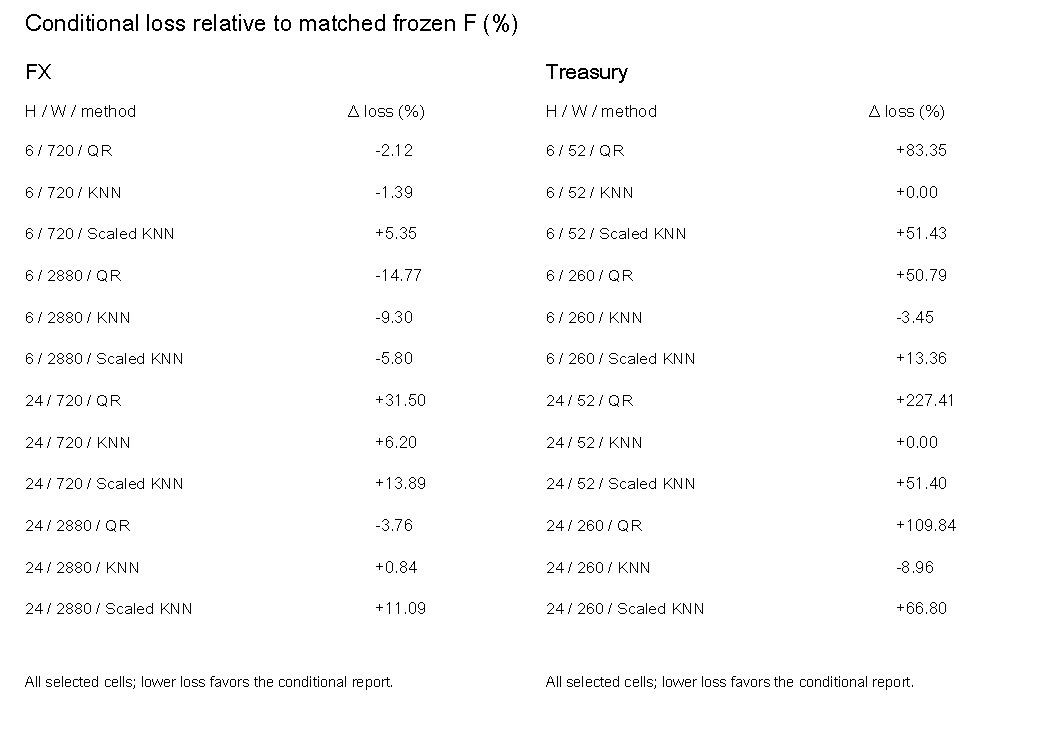
\includegraphics[width=.96\linewidth]{figures/conditional-common-history.pdf}
Figure S1. All 24 selected conditional forecasts versus frozen F with the same source, horizon, history window and refit schedule. Entries show within-reference mean-loss percentages; negative favors the conditional procedure. Source panels have explicit scales and are not pooled. Full-pool KNN identities are marked.
\end{figure}
\begin{figure}[htbp]
\centering
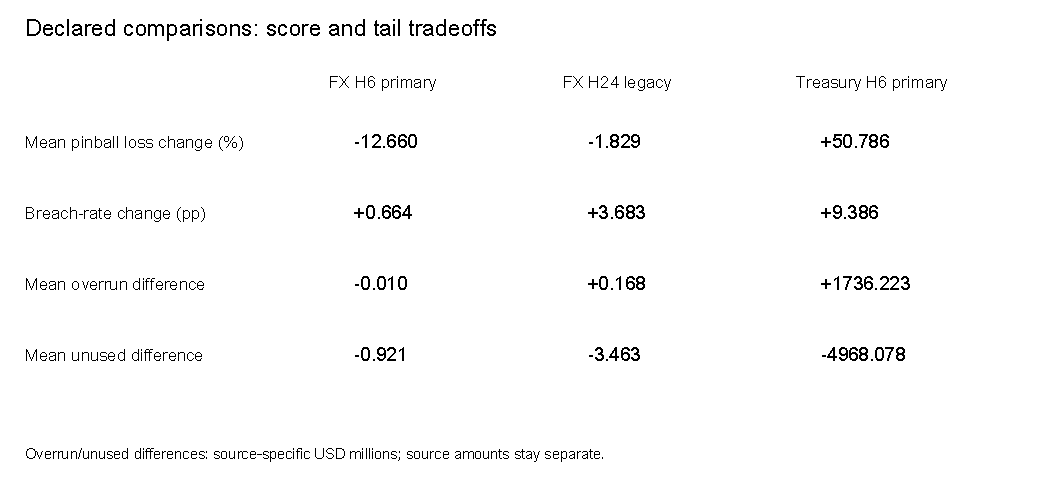
\includegraphics[width=.96\linewidth]{figures/conditional-primary-tradeoffs.pdf}
Figure S2. The two declared source primaries and FX H24 legacy-reference sensitivity: relative mean-loss, underprediction and overprediction changes, plus breach-rate differences in percentage points. These are separate descriptive quantities, separate measures of forecast behavior. A reduced overprediction amount is not automatically overall improvement.
\end{figure}
\begin{figure}[htbp]
\centering
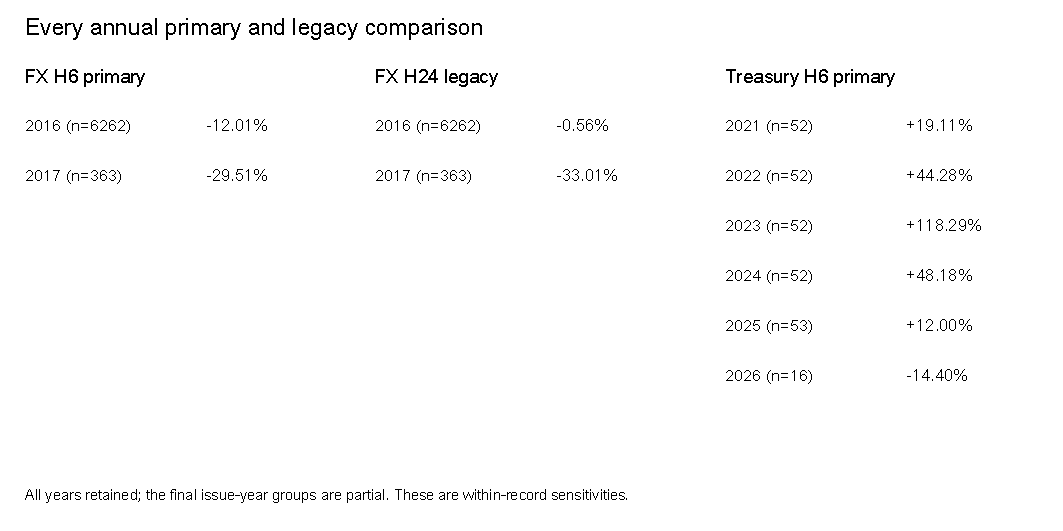
\includegraphics[width=.96\linewidth]{figures/conditional-annual-primary.pdf}
Figure S3. Every issue-year group for the two declared primaries and FX H24 legacy sensitivity. Values are paired within-reference loss percentages, with origin counts and partial years labeled. They are subdivisions of the same source records, not independent replications, confidence intervals or retrospectively selected switching regimes.
\end{figure}
\begin{figure}[htbp]
\centering
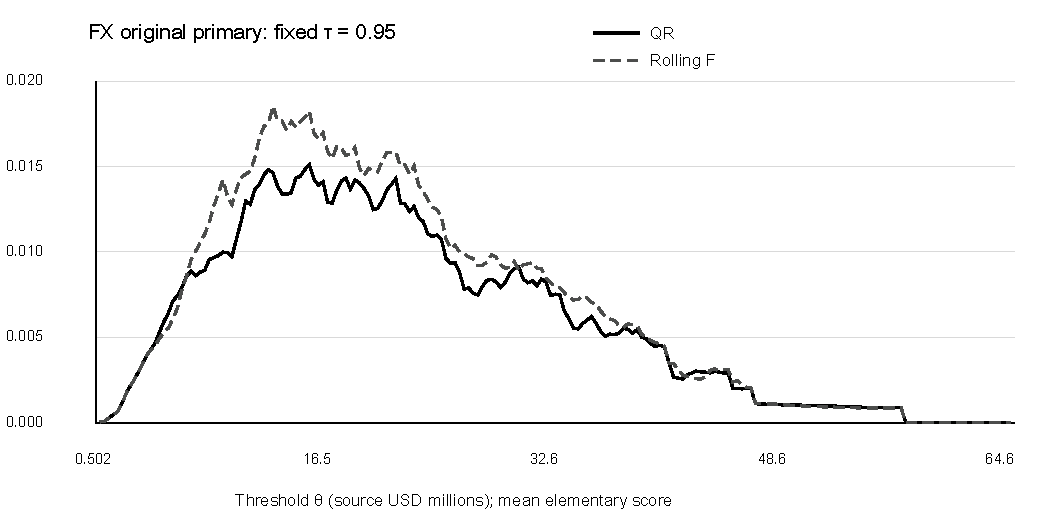
\includegraphics[width=.96\linewidth]{figures/murphy-fx_hourly.pdf}
Figure S4\(\dagger\). FX original primary elementary quantile scores at fixed \(\tau=0.95\). Lower is better. The full-breakpoint check finds crossing; the display grid alone is not used to support that finding.
\end{figure}
\begin{figure}[htbp]
\centering
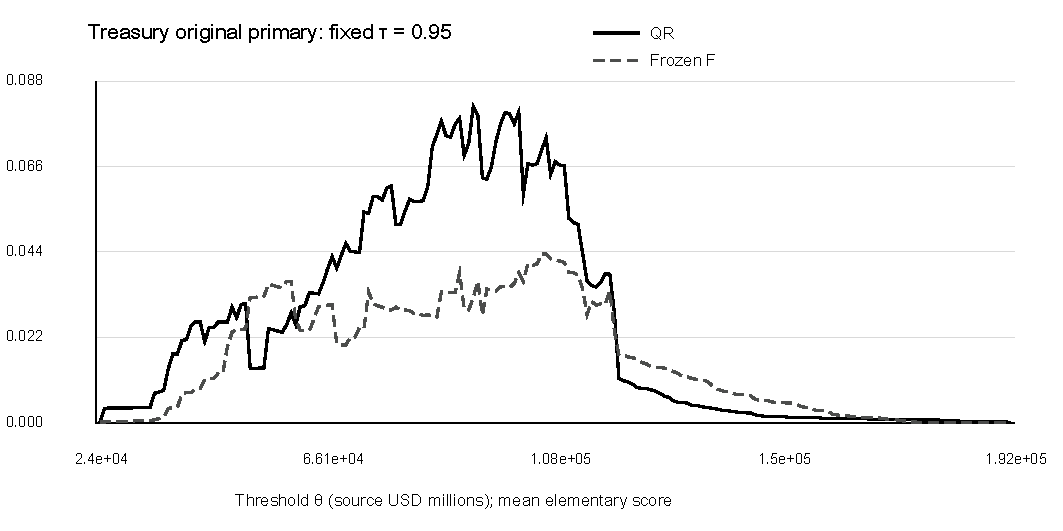
\includegraphics[width=.96\linewidth]{figures/murphy-nyfed_weekly.pdf}
Figure S5\(\dagger\). Treasury original primary elementary quantile scores at fixed \(\tau=0.95\). Lower is better. The full-breakpoint check finds crossing; the display grid alone is not used to support that finding.
\end{figure}
\section*{S15. V5 post-result analyses and positioning evidence}
\subsection*{Chronological budgets retained from the main article}
\begingroup\footnotesize
\begin{samepage}Table S36. Frozen source-specific chronological budgets. All indices are zero based; W and d count source records. H is 6 or 24 in every cell.\end{samepage}
\begin{longtable}{>{\raggedright\arraybackslash}p{0.192\linewidth}>{\raggedright\arraybackslash}p{0.192\linewidth}>{\raggedright\arraybackslash}p{0.192\linewidth}>{\raggedright\arraybackslash}p{0.192\linewidth}>{\raggedright\arraybackslash}p{0.192\linewidth}}
\toprule
Source & Validation origins & Evaluation origins & W & Refit d \\
\midrule
\endhead
FX & 10463--11902 (1440) & 11927--18551 (6625) & 720 / 2880 & 24 \\
Treasury & 329--380 (52) & 405--681 (277) & 52 / 260 & 13 \\
\bottomrule
\end{longtable}
\endgroup
\subsection*{Deliberately immature-label oracle}
A deliberately invalid label-timing control retains the original selected parameters, long history and refit clock on predetermined first, middle and last complete blocks: 72 FX origins and 39 Treasury origins. Replacing the clean pool ending at r\(-\)H with one ending at r includes 6 immature labels per refit. In Treasury QR the illegal oracle reduces loss by 33.3988\% but changes breaches from 5 to 6; FX QR instead raises loss by 0.0639\%. The complete QR, KNN and F outcomes in Supplement Table S37 have mixed directions. This post-result / exploratory control quantifies timing contamination in these blocks, not an inevitable optimism bias or an all-sample performance effect.

\begingroup\footnotesize
\begin{samepage}Table S37\(\dagger\). Deliberately immature-label oracle versus clean training on the first, middle and last complete original refit blocks. FX has 72 origins and Treasury 39; each refit adds 6 illegal labels. Source units are USD for FX and USD millions for Treasury. The oracle-minus-clean percentage has the clean loss as denominator. These are selected clock blocks, not the full evaluation sample; the oracle is not deployable.\end{samepage}
\begin{longtable}{>{\raggedright\arraybackslash}p{0.160\linewidth}>{\raggedright\arraybackslash}p{0.160\linewidth}>{\raggedright\arraybackslash}p{0.160\linewidth}>{\raggedright\arraybackslash}p{0.160\linewidth}>{\raggedright\arraybackslash}p{0.160\linewidth}>{\raggedright\arraybackslash}p{0.160\linewidth}}
\toprule
Source & Method & Clean loss & Illegal loss & Illegal \(\Delta\)\% & Breaches C/O \\
\midrule
\endhead
FX & QR & 254,757.369210 & 254,920.239898 & +0.063932 & 2 / 2 \\
FX & KNN & 294,045.707972 & 297,278.423087 & +1.099392 & 2 / 3 \\
FX & F & 259,673.056354 & 259,673.056354 & +0.000000 & 0 / 0 \\
Treasury & QR & 3,128.675515 & 2,083.734631 & \(-\)33.398826 & 5 / 6 \\
Treasury & KNN & 1,759.683333 & 1,713.746154 & \(-\)2.610537 & 0 / 0 \\
Treasury & F & 1,615.698718 & 1,640.832051 & +1.555571 & 2 / 2 \\
\bottomrule
\end{longtable}
\endgroup
The clean and illegal arms keep selected parameters fixed; transforms are recomputed within each arm. The blocks are deterministic clock locations rather than favorable outcome selections. Clean stored outputs are independently read back from the original hash-bound trace subset, but this is an implementation check on the same data, not independent financial validation.

\subsection*{Exact gain bridge}
main-article Table 5 expresses the original FX primary gain as an exact descriptive bridge: the joint history/update contrast adds +2.4716 percentage points, and the conditional-procedure contrast adds \(-\)15.1317, using the same original-reference denominator. Their sum is \(-\)12.6601\%. The separate matched-reference percentage is \(-\)14.7668\%; adding it to the first bridge entry would mix denominators. History length and update frequency change together in the first step; features, estimation and procedure change in the second. This post-result / exploratory arithmetic identifies no isolated causal effect.

\subsection*{Mathematical illustrations}
The construction properties are elementary target-specific statements, not newly discovered probability inequalities. Exact finite-distribution checks show that identical marginal observations and identical endpoint marginals need not determine a peak quantile. A separate counterexample rejects substitution of a one-sided endpoint quantile for the absolute-displacement quantile. The executable examples, floor-atom counterexample and raise-only horizon-repair counterexample are retained in the theory source and tests.

Artificial marginal example. At each of two future observation times, the position is 1 with probability 3/100 and 0 otherwise, starting from 0. Aligning the two positive events gives peak probability 3/100; making them disjoint gives 3/50. Each time marginal, including the endpoint, is identical across the two constructions. At quantile level 19/20, their peak quantiles are respectively 0 and 1. Thus endpoint or even all individual-time marginals do not identify the peak quantile without the temporal joint distribution.

Artificial endpoint-quantile substitution example. Independent increments have X\textsubscript{1}=0 with probability 23/25, X\textsubscript{1}=\(-\)3 or 3 each with probability 1/25, and X\textsubscript{2}=\(-\)1 or 1 each with probability 1/2. At level 39/40, the signed endpoint quantile is 2, whereas the absolute endpoint quantile is 4. Starting at 0, the sampled-peak probability above the signed threshold is 2/25, exceeding nominal 1/20. The increments satisfy independence and symmetry: the failure is the substitution of the wrong endpoint functional.

Artificial floor and horizon examples. A uniform outcome on [B,B+1] satisfies the floor but has no atom at B. For ordered true outcomes (1,1) and reports (2,1), a raise-only long-horizon repair gives (2,2). At \(\tau=19/20\), long-horizon pinball loss rises from 0 to 1/20; the short report is unchanged. This rejects an unconditional guarantee for that raise-only repair, not for every monotone rearrangement.

A raise-only horizon repair can increase loss; this does not imply that every monotone rearrangement fails. Under a common quantile level, equal weights and ordered outcomes, sorting can weakly improve the total pinball sum without ensuring improvement separately at every horizon.

\subsection*{Positioning-table original-text evidence}
The following source locators apply to the reported cell values. n.r. means not reported in the actual inspected scope, rather than a verified absence throughout an entire work. The original thesis on conditional cash peaks could not be newly retrieved and is omitted from the table rather than assigned guessed cells.

\textbf{Wisniewski et al. (2020); Wisniewski (2024).} Forecast object: Signed endpoint interval (W20, §1, physical p2; W24, §6.1, physical p108 / printed p107). Data unit: One FX dealer (W20, §3.1, physical p4; W24, §2.4, physical p34 / printed p33; §6.3.1, p111 / p110). Known peak floor: Peak floor n.r. (W20, §2, physical pp3--4; §§3.3--3.4, pp7--8; W24, §6.2, physical pp109--111 / printed pp108--110). Outcome maturity / ordering: Ordered endpoint split; peak n.r. (W20, §2 / Fig1, physical p3; §3.2, p7; W24, §6.2 / Fig6.1, physical pp109--110; §6.3.2, pp112--113). Evaluation: Pinball/Winkler; UC/CC (W20, §3.5, physical pp9--10; §4.3, p14; W24, §6.3.5, physical pp118--119; §6.4.3 / Table6.2, p124). Cross-source scope: n.r. in endpoint task (W20, §3.1 and §4, physical pp4,11--15; W24, §6.3.1 and §§6.4--6.5, physical pp111,119--125).

\textbf{Boudoukh et al. (2004).} Forecast object: Worst portfolio return (MAX\_FINAL, §2, physical/printed pp2--3). Data unit: Stylized fixed portfolio (MAX\_FINAL, §§1--2, p2). Known peak floor: Initial value known; peak floor n.r. (MAX\_FINAL, §2, pp2--3). Outcome maturity / ordering: n.r.; analytic/simulation (MAX\_FINAL, §§2--3, pp2--4). Evaluation: Tail probability; VaR ratios (MAX\_FINAL, §3 / Tables1--2, pp3--5). Cross-source scope: n.r.; parameter cases (MAX\_FINAL, §§3--4, pp3--5).

\textbf{Petrunia et al. (2019).} Forecast object: Daily cross-participant debit maximum (petrunia2019, p.8 §2; p.13 §4b). Data unit: ACSS clearers (petrunia2019, p.8 §2). Known peak floor: Peak floor n.r. (petrunia2019, pp.9--11 §3). Outcome maturity / ordering: Incoming-data updates; peak n.r. (petrunia2019, p.13 §4b). Evaluation: Tail fit; collateral shortfalls (petrunia2019, pp.10--13 §§3c,4,4b). Cross-source scope: Within ACSS; source transfer n.r. (petrunia2019, pp.13--14 §4b).

\textbf{Arjani et al. (2020).} Forecast object: Remaining-day liquidity ratio (arjani2020, printed pp.7--9 §3.1 eqs.1--5). Data unit: LVTS participants (arjani2020, printed p.12 §3.2.2). Known peak floor: Known flows; peak floor n.r. (arjani2020, printed pp.7--9 eqs.1--5). Outcome maturity / ordering: Chronological split; peak n.r. (arjani2020, printed pp.12--13 §3.2.2). Evaluation: RMSE; liquidity-risk bands (arjani2020, printed pp.12--13,20 §§3.2.2--3.3). Cross-source scope: Within LVTS; source transfer n.r. (arjani2020, printed pp.12,20).

\textbf{Engle--Manganelli (2004).} Forecast object: Conditional return quantile (engle2004, pp.368--369 §3 eqs.1--4). Data unit: Stocks and index returns (engle2004, p.371 §6). Known peak floor: Peak floor n.r. (engle2004, pp.368--369 §3). Outcome maturity / ordering: Lagged predictors; held-out returns (engle2004, pp.368,371 §§3,6; p.375 App.A DQ8). Evaluation: Quantile objective; hits; DQ (engle2004, pp.371--373 §6,Table1). Cross-source scope: Several returns; different task (engle2004, p.371 §6).

\textbf{Ehm et al. (2016).} All Ehm page locators below refer to the arXiv author-v2 revision, not final journal pagination. Forecast object: Quantile/expectile ranking (ehm2016, §§3.2--3.4 pp.15--20). Data unit: Survey, probability and wind cases (ehm2016, §§4.1--4.3 pp.22--25). Known peak floor: Zero wind support; moving peak floor n.r. (ehm2016, §4.3 p.25). Outcome maturity / ordering: Original splits; peak n.r. (ehm2016, §4.3 p.25). Evaluation: Murphy; coverage/sharpness (ehm2016, §4.3 pp.25--26; §3.4 p.20). Cross-source scope: Multiple domains; different tasks (ehm2016, §4 pp.22--26).

\textbf{Duffie et al. (2023).} Forecast object: Capacity/illiquidity; PnL VaR (duffie2023, §1 printed pp.1--4; §6 pp.24--27). Data unit: Dealer and market sources (duffie2023, §1 pp.2--4; App.E pp.58--59). Known peak floor: Peak floor n.r. (duffie2023, §1 pp.3--4). Outcome maturity / ordering: Expanding VaR; peak n.r. (duffie2023, App.E p.58,fn27). Evaluation: Quantile fit; PnL forecasts (duffie2023, §6 pp.24--27; App.E pp.58--59). Cross-source scope: Several sources; different task (duffie2023, §1 pp.2--4; App.E pp.58--59).

\textbf{This study.} Forecast object: Sampled absolute peak (THIS\_STUDY, ['sections', 3, 'blocks', 2]). Data unit: One FX dealer; Treasury totals (THIS\_STUDY, ['sections', 2]). Known peak floor: Observed \(|N_t|\) projection (THIS\_STUDY, ['sections', 3, 'blocks', 16]). Outcome maturity / ordering: Completed peak labels (THIS\_STUDY, ['sections', 3, 'blocks', 0]). Evaluation: Pinball; coverage; Murphy (THIS\_STUDY, ['sections', 4]). Cross-source scope: FX and related Treasury tasks (THIS\_PANEL, eligible; THIS\_STUDY, sections[7].blocks[5]). Treasury task count: 13 = 1 original bill + 12 related additional aggregates; not independent dealers.

Source IDs identify the original links and actual reading ranges in the repository source register and novelty-search log. The excluded cash-peak thesis remains a narrative precedent; failed current access is not evidence that a concept is absent.

\section*{References}
Arjani, N., F. Li and L. Sabetti (2020). Monitoring Intraday Liquidity Risks in a Real Time Gross Settlement System. Payments Canada discussion paper. \href{https://www.payments.ca/sites/default/files/discussion_paper_monitoring_intraday_liquidity_risks_in_a_real_time_gross_settlement_system.pdf}{official report}.

Barone-Adesi, G., K. Giannopoulos and L. Vosper (1999). VaR without correlations for portfolios of derivative securities. \emph{Journal of Futures Markets} 19(5), 583--602. DOI:10.1002/(SICI)1096-9934(199908)19:5\( < \)583::AID-FUT5\( > \)3.0.CO;2-S.

Boudoukh, J., M. Richardson, R. Stanton and R.F. Whitelaw (2004). MaxVaR: Long-Horizon Value at Risk in a Mark-to-Market Environment. Journal of Investment Management 2(3),1--6. Author-hosted final-layout article. \href{https://pages.stern.nyu.edu/~rwhitela/papers/maxvar\%20joim04.pdf}{Original source}.

Boyd, S., N. Parikh, E. Chu, B. Peleato and J. Eckstein (2011). Distributed Optimization and Statistical Learning via the Alternating Direction Method of Multipliers. \emph{Foundations and Trends in Machine Learning} 3(1), 1--122. \href{https://doi.org/10.1561/2200000016}{DOI:10.1561/2200000016}. \href{https://web.stanford.edu/~boyd/papers/pdf/admm_distr_stats.pdf}{author PDF}.

Casgrain, P., M. Larsson and J. Ziegel (2023). Anytime-valid sequential testing for elicitable functionals via supermartingales. \href{https://arxiv.org/abs/2204.05680v2}{arXiv:2204.05680v2}, 4 June.

Christoffersen, P.F. (1998). Evaluating Interval Forecasts. \emph{International Economic Review} 39(4), 841--862. \href{https://doi.org/10.2307/2527341}{DOI}.

Duffie, D., M. Fleming, F. Keane, C. Nelson, O. Shachar and P. Van Tassel (2023). Dealer Capacity and U.S. Treasury Market Functionality. Federal Reserve Bank of New York Staff Report No. 1070, August, revised October. \href{https://doi.org/10.59576/sr.1070}{DOI:10.59576/sr.1070}. \href{https://www.newyorkfed.org/medialibrary/media/research/staff_reports/sr1070.pdf}{official report}.

Ehm, W., T. Gneiting, A. Jordan and F. Krüger (2016). Of quantiles and expectiles: consistent scoring functions, Choquet representations and forecast rankings. Journal of the Royal Statistical Society: Series B 78(3),505--562. DOI:10.1111/rssb.12154. Consulted author preprint: arXiv:1503.08195v2 (2015 revision). \href{https://doi.org/10.1111/rssb.12154}{Original source}.

Engle, R.F. and S. Manganelli (2004). CAViaR: Conditional Autoregressive Value at Risk by Regression Quantiles. \emph{Journal of Business \& Economic Statistics} 22(4), 367--381. \href{https://doi.org/10.1198/073500104000000370}{DOI:10.1198/073500104000000370}.

Gneiting, T. (2011). Making and Evaluating Point Forecasts. \emph{Journal of the American Statistical Association} 106(494), 746--762. \href{https://doi.org/10.1198/jasa.2011.r10138}{DOI:10.1198/jasa.2011.r10138}.

Henzi, A. and J.F. Ziegel (2022). Valid sequential inference on probability forecast performance. \href{https://arxiv.org/abs/2103.08402v3}{arXiv:2103.08402v3}, 1 July.

Hull, J. and A. White (1998). Incorporating volatility updating into the historical simulation method for value-at-risk. \emph{Journal of Risk} 1(1), 5--19. \href{https://doi.org/10.21314/jor.1998.001}{DOI:10.21314/jor.1998.001}.

McNeil, A.J., and Frey, R. (2000). Estimation of tail-related risk measures for heteroscedastic financial time series: an extreme value approach. \emph{Journal of Empirical Finance}7(3--4),271--300. \href{https://doi.org/10.1016/S0927-5398(00)00012-8}{DOI:10.1016/S0927-5398(00)00012-8}.

Petrunia, R., L. Sabetti and M. Voia (2019). Tail Risk in the Automated Clearing Settlement System (ACSS). Payments Canada Discussion Paper No. 7, January 2019 update of September 2018 original. \href{https://www.paiements.ca/sites/default/files/tail_risk_in_the_automated_clearing_settlement_system_acss.pdf}{official discussion paper}.

Politis, D.N. and J.P. Romano (1994). The Stationary Bootstrap. \emph{Journal of the American Statistical Association} 89(428), 1303--1313. \href{https://doi.org/10.1080/01621459.1994.10476870}{DOI:10.1080/01621459.1994.10476870}.

Wisniewski, W. (2024). \emph{Net Position and Retail Trader Behaviour: Implications for Market Makers' Risk Management Strategies}. Doctoral thesis, Royal Holloway, University of London. \href{https://pure.royalholloway.ac.uk/en/publications/net-position-and-retail-trader-behaviour-implications-for-market-/}{Institutional record}.

Wisniewski, W., D. Lindsay and S. Lindsay (2020). Application of Conformal Prediction Interval Estimations to Market Makers' Net Positions. Proceedings of the Ninth Symposium on Conformal and Probabilistic Prediction and Applications, \emph{Proceedings of Machine Learning Research} 128, 285--301. \href{https://proceedings.mlr.press/v128/wisniewski20a.html}{Official proceedings}.

\section*{Figure captions}
Figure S1. All 24 selected conditional forecasts versus frozen F with the same source, horizon, history window and refit schedule. Entries show within-reference mean-loss percentages; negative favors the conditional procedure. Source panels have explicit scales and are not pooled. Full-pool KNN identities are marked.

Figure S2. The two declared source primaries and FX H24 legacy-reference sensitivity: relative mean-loss, underprediction and overprediction changes, plus breach-rate differences in percentage points. These are separate descriptive quantities, separate measures of forecast behavior. A reduced overprediction amount is not automatically overall improvement.

Figure S3. Every issue-year group for the two declared primaries and FX H24 legacy sensitivity. Values are paired within-reference loss percentages, with origin counts and partial years labeled. They are subdivisions of the same source records, not independent replications, confidence intervals or retrospectively selected switching regimes.

Figure S4\(\dagger\). FX original primary elementary quantile scores at fixed \(\tau=0.95\). Lower is better. The full-breakpoint check finds crossing; the display grid alone is not used to support that finding.

Figure S5\(\dagger\). Treasury original primary elementary quantile scores at fixed \(\tau=0.95\). Lower is better. The full-breakpoint check finds crossing; the display grid alone is not used to support that finding.

\end{document}
